\documentclass[msc,numbers]{coppe}
\usepackage[utf8]{inputenc}
\usepackage{amsmath,amssymb, mathtools}
\usepackage{hyperref}
\usepackage{indentfirst}
\usepackage{graphics}
\usepackage{float}
\usepackage{algpseudocode,algorithm}
%%%%%%%%%%%%%%%%%%%%%%%%%%%%%%%%%%%%%%%%%%%%%%%%%%%%%%%%%%%%%%%%%%%%%%%%%%%%%%%%%%%%%%%%%%%%%%%%
% Declarações em Português do Pseudocódigo
\algrenewcommand\algorithmicend{\textbf{fim}}
\algrenewcommand\algorithmicdo{\textbf{faça}}
\algrenewcommand\algorithmicwhile{\textbf{enquanto}}
\algrenewcommand\algorithmicfor{\textbf{para}}
\algrenewcommand\algorithmicforall{\textbf{para cada}}
\algrenewcommand\algorithmicif{\textbf{se}}
\algrenewcommand\algorithmicthen{\textbf{então}}
\algrenewcommand\algorithmicelse{\textbf{senão}}
\algrenewcommand\algorithmicreturn{\textbf{devolve}}
\algrenewcommand\algorithmicfunction{\textbf{função}}
\algrenewtext{EndWhile}{\algorithmicend\ \algorithmicwhile}
\algrenewtext{EndFor}{\algorithmicend\ \algorithmicfor}
\algrenewtext{EndIf}{\algorithmicend\ \algorithmicif}
\algrenewtext{EndFunction}{\algorithmicend\ \algorithmicfunction}
\algnewcommand\algorithmicto{\textbf{até}}
\algrenewtext{For}[3]%
{\algorithmicfor\ #1 $\gets$ #2 \algorithmicto\ #3 \algorithmicdo}
\makeatletter
\newcommand{\newalgname}[1]{%
  \renewcommand{\ALG@name}{#1}%
}
\newalgname{Algoritmo}% All algorithms will be called "Algoritmo"
\renewcommand{\listalgorithmname}{Lista de \ALG@name s}
\makeatother
%%%%%%%%%%%%%%%%%%%%%%%%%%%%%%%%%%%%%%%%%%%%%%%%%%%%%%%%%%%%%%%%%%%%%%%%%%%%%%%%%%%%%%%%%%%%%%%%
\newcommand{\argmin}{\arg\!\min}
\newcommand{\argmax}{\arg\!\max}
\newcommand*\rfrac[2]{{}^{#1}\!/_{#2}}

\makelosymbols
\makeloabbreviations

\begin{document}
  \title{Aprendizado Ativo aplicado à Elicitação de Preferências para fins de Incentivo}
  \foreigntitle{Active Learning applied to Rating Elicitation for Incentives Purposes}
  \author{Marden Braga}{Pasinato}
  \advisor{Prof.}{Geraldo Zimbrão da}{Silva}{D.Sc.}
  %\advisor{Prof.}{Carlos Eduardo}{Ribeiro de Mello}{D.Eng.}
  %\advisor{Prof.}{Nome do Terceiro Orientador}{Sobrenome}{D.Sc.}

  \examiner{Prof.}{Geraldo Zimbrão da Silva}{D.Sc.}
  \examiner{Prof.}{Geraldo Bonorino Xexéo}{D.Sc.}
  \examiner{Prof.}{Leandro Guimarães Marques Alvim}{D.Sc.}
  \examiner{Prof.}{Carlos Eduardo Ribeiro de Mello}{D.Sc.}
  %\examiner{Prof.}{Nome do Quarto Examinador Sobrenome}{Ph.D.}
  %\examiner{Prof.}{Nome do Quinto Examinador Sobrenome}{Ph.D.}
  \department{PESC}
  \date{11}{2014}

  \keyword{Sistemas de Recomendação}
  \keyword{Aprendizado Ativo}
  \keyword{Elicitação de Preferências}
  
  %\abbrev{SR}{Sistema de Recomendação}
  %\abbrev{AM}{Aprendizado de Máquina}
  %\abbrev{AA}{Aprendizado Ativo}

  \maketitle

  \frontmatter
  \include{dedic}
  \chapter*{Agradecimentos}

Em toda caminhada longa e árdua, há momentos de tropeço e desânimo que só são superados quando alguém lhe estende a mão e lhe coloca novamente no caminho. No meu caso não foi diferente, portanto, tenho muitas mãos a agradecer.

Agradeço ao meu orientador, prof. Geraldo Zimbrão, por acreditar no meu potencial e pela orientação deste trabalho. Minha gratidão aos membros da banca pelo tempo e atenção devotados à análise desta dissertação. Em especial, ao prof. Carlos Mello, cujas ideias e conselhos foram fundamentais, não apenas em minha vida acadêmica, mas também em minha vida pessoal. Cadu, se assim me permite, meu muito obrigado.

Quero agradecer aos meus amigos do PESC, que, entre um café e outro, me deram dicas de leitura; apontaram meus erros; apludiram meus acertos; me deram caronas; me contaram piadas; escutaram pacientemente minhas angústias e alegrias. Braida, Duarte, Horta, Luis e Pedro, não sei se aguentaria sem vocês.

Não posso deixar de agradecer ao prof. Daniel Figueiredo que, desde da graduação, me motivou a entrar no mundo acadêmico e, durante o mestrado, sempre se mostrou solicito a escutar meus problemas e pensar em soluções. Agradeço também a todos os funcionários do PESC e da CAPES por proverem uma infraestrutura onde pude me apoiar.

Sem dúvida, o maior auxílio que tive foi o amor e suporte da minha família. Não só agradeço, como também dedico este trabalho a eles: meus pais, minha irmã, meus avós, meus tios e primos. Meu muito obrigado pelo carinho; pelas palavras de ternura; pela compreensão e pelos tantos ``vai dar tudo certo''.

Por último, mas não menos importante, agradeço à mão que me pôs de pé após as quedas mais dolorosas e angustiantes. Obrigado Deus, por tudo!
  \begin{abstract}

Na literatura de Sistemas de Recomendação, estratégias de Aprendizado Ativo foram extensamente aplicadas à elicitação preferências para amenizar os efeitos do Arranque Frio, tarefa conhecida como \textit{Elicitação de Preferências para fins de Arranque Frio}. Contudo, se soubéssemos quais são os $N$ itens, dentre os já adquiridos mas não avaliados, que, se avaliados, trarão o maior ganho para o sistema em termos de acurácia, valeria a pena oferecer um incentivo para que o usuário avalie tais itens. A esta tarefa damos o nome de \textit{Elicitação de Preferência para fins de Incentivo}.

Este trabalho propõe uma nova estratégia de Aprendizado Ativo, que seleciona os itens com base na distribuição de probabilidade dos mesmos, gerando um conjunto de treinamento sem viés. A batizada \textit{Estratégia Livre de Viés} foi comparada com outras 16 estratégias populares dentro da literatura no que diz respeito a \textit{Elicitação de Preferência para fins de Incentivo}. A \textit{Estratégia Livre de Viés} mostrou desempenho superior as demais em termos de acurácia global do sistema. Além disso, apresentamos uma análise do comportamento de cada estratégia, levando em consideração os possíveis motivos de seu sucesso ou fracasso. 

\end{abstract}


  \begin{foreignabstract}

In the literature of Recommender Systems, Active Learning strategies have been extensively applied to rating elicitation in order to mitigate Cold Start effects, namely \textit{Rating Elicitation for Cold Start Purposes}. However, if we knew the best $N$ items, among those already acquired but not evaluated, which, if evaluated, would result in the greatest improvement in terms of overall system's accuracy, it would probably be worthwhile to give users an incentive for evaluating those items. We call this task \textit{Rating Elicitation for Incentives Purposes}. 

This work proposes a novel Active Learning strategy that selects items based on their probability distribution, creating an unbiased training set. The so called \textit{Unbiased Strategy} was compared with other 16 popular strategies in the literature concerning \textit{Rating Elicitation for Incentives Purposes}. The \textit{Unbiased Strategy} outperformed  the others in terms of overall system's accuracy. Moreover, we present an analysis of each strategy's performance, taking into account the possible reasons for their success or failure.

\end{foreignabstract}


  \tableofcontents
  \listoffigures
  \listoftables
  \listofalgorithms
  \addcontentsline{toc}{chapter}{\listalgorithmname}
  \printlosymbols
  \printloabbreviations
  %\addcontentsline{toc}{chapter}{\listabbreviationname}

  \mainmatter
  \chapter{Introdução}
\section{Motivação}

Há uma frase, de autor desconhecido, mas que ficou muito famosa, com o dizer: ``informação é o novo petróleo''. Apesar do conteúdo sensacionalista, não é possível negar que a veracidade da mesma vem se confirmando nas últimas décadas. De fato, nunca se produziu tanta informação em toda história e, ao mesmo tempo, nunca se dependeu tanto da mesma. As maneiras habituais de trabalho, estudo, locomoção, relacionamento e convívio foram completamente remodeladas, passando a ser fortemente informatizadas. Ou seja, os indivíduos estão cada vez mais dependentes de aparatos tecnológicos para executar tarefas antes consideradas básicas e triviais. Tal fenômeno chamou a atenção dos pesquisadores que o batizaram de \textit{Era da Informação} \citep{castells_information_1999}.

Existem muitas vantagens e desvantagens associadas à tal Era da Informação, assim como em tudo o mais. No entanto, uma de suas mais aclamadas vantagens está se transformando em uma desvantagem. Boa parte desta sobrecarga de informação se encontra atualmente na Internet, o que cria uma enorme oferta de opções para os usuários. A intuição comum normalmente associa variedade à satisfação, isto é, quanto mais opções um usuário tiver, consequentemente, mais satisfeito ele estará. Contudo, o que se observa na prática é que, frente a um demasiado numero opções, os usuários se angustiam, uma vez que o risco de fazer a escolha errada aumenta consideravelmente. Portanto, a exacerbada variedade de opções vem causando descontentamento ao invés de satisfação \citep{schwartz_paradox_2004}.

Este paradoxo torna-se mais visível quando consideramos o comércio eletrônico, também conhecido como \textit{e-commerce}. Uma das esferas da vivência humana mais afetada pela Era da Informação foi, sem dúvida, o comércio. Chega a ser difícil encontrar uma empresa que não oferte seus produtos \textit{online}. Por outro lado, a Internet deixou de ser apenas mais um canal de comunicação com o cliente e passou a ser o habitat natural de novos negócios, muitos deles comercializando bens intangíveis (e.g., \textit{software}, áudio, vídeo, etc.), que são facilmente armazenáveis. Some-se a isto o fato de que as lojas virtuais, quando ofertam bens tangíveis, isto é, produtos físicos em geral, não precisam tê-los em estoque no momento da venda. Tais fatores conferem aos \textit{e-commerces} uma enorme flexibilidade para montar seus catálogos, que podem atingir facilmente a ordem de milhões de itens.

Comprar, por sua vez, nunca foi uma ação tão simples e, ao mesmo tempo, tão complexa. Simples no sentido de que a revolução informacional acabou criando formas mais eficientes de pagamentos e, hoje, é possível literalmente comprar uma grande quantidade de itens com apenas um \textit{click}. Entretanto, escolher o que comprar se tornou uma tarefa complexa tendo em vista as inúmeras possibilidades oferecidas \textit{online}. O usuário comum se depara com uma infinidade de lojas virtuais, de toda parte do globo, cada uma com um catálogo praticamente ilimitado de itens. Não é atoa que estão surgindo diversos serviços voltados somente para auxiliar o usuário a encontrar o que deseja, como, por exemplo, buscadores específicos para produtos, comparadores de preço, atendimento virtual, entre outros.

Dentre as ferramentas que visam auxiliar o usuário durante a compra, nenhuma chamou tanto a atenção da indústria quanto os Sistemas de Recomendação (SR). Durante as últimas duas décadas, as grandes empresas da Internet investiram fortemente em tais sistemas, pois perceberam que o usuário se sente perdido em meio a tantas opções e, no fim, acaba por desistir da compra. Ao oferecer recomendações, o sistema pretende amenizar a dúvida do usuário, reduzindo o número de opções a se considerar. Ademais, a loja virtual passa a sensação de que compreende o usuário, ou seja, que sabe distinguir entre os itens que ele gosta e os que ele não gosta. 

%\abbrev{SR}{Sistema de Recomendação}

Além de, claro, aumentar a probabilidade de venda ao recomendar os itens que o usuário gosta (ou pelo menos que o site acredita que ele gosta), a sensação de ser atendido de forma personalizada estabelece, em muitos usuários, uma relação de confiança. Em outras palavras, SR não servem apenas para alavancar vendas, podem ser concebidos como uma forma de se estreitar o relacionamento com o cliente \citep{Schafer:1999:RSE:336992.337035}.

A academia, por sua vez, também investiu com veemência no aprimoramento das técnicas de recomendação. Em especial, a competição organizada pelo \textit{Netflix} trouxe muita atenção para este tema, uma vez que levou pesquisadores de todo o mundo a trabalharem em um algoritmo que fosse mais eficiente que o do próprio \textit{Netflix} \citep{Bennett07thenetflix}. Como resultado, diversos algoritmos foram propostos, a grande maioria se baseando em métodos de Aprendizado de Máquina (AM) e Data Mining (DM), o que trouxe importantes avanços para a área \citep{Bell:2007:LNP:1345448.1345465, ricci_recommender_2011}.

%\abbrev{AM}{Aprendizado de Máquina}
%\abbrev{DM}{Data Mining}

Em geral, as técnicas de recomendação podem ser divididas em três abrangentes categorias: Baseadas em Contexto (BC), Filtragem Colaborativa (FC) e Híbridas. No capítulo \ref{cap:fundamentacao}, iremos descrever em detalhes cada uma dessas categorias e as principais técnicas de cada uma. Por hora, é suficiente mencionar que as técnicas de FC se sobressaem às demais, principalmente em termos de desempenho e aplicabilidade. No entanto, elas sofrem com o problema do \textit{Arranque Frio} (AF), ou problema do \textit{Novo Usuário/Item}. Como muitas delas se baseiam em noções de similaridade entre usuários/itens, extraídas a partir das preferências dos usuários, não é possível calcular nenhuma recomendação para o novo usuário/item, visto que não se pode medir sua similaridade para com os demais usuários/itens \citep{su_survey_2009}.

%\abbrev{FC}{Filtragem Colaborativa}
%\abbrev{AF}{Arranque Frio}

Por esta razão, muitos trabalhos foram propostos na tentativa de amenizar o problema do AF em FC, sobretudo no tocante ao novo usuário \citep{Rashid:2002:GKY:502716.502737, Rashid:2008:LPN:1540276.1540302, elahi_rating_2011, elahi_system-wide_2011, Elahi:2014:ALS:2542182.2542195}. Tais propostas buscam aumentar o conhecimento do sistema sobre os novos usuários, solicitando aos mesmos que deem suas preferências (na forma de avaliações) para alguns itens previamente definidos. A este processo, que precede o cálculo das recomendações, damos o nome de \textit{Elicitação de Preferências}.

É importante delinear que a Elicitação de Preferências pode ser utilizada em contextos que não são necessariamente relacionados ao problema de AF. Infelizmente, na literatura, esses termos podem parecer sinônimos, uma vez que a grande maioria dos trabalhos envolvendo Elicitação de Preferências são voltados para contornar as deficiências geradas pelo AF. A fim de distinguir os cenários onde o processo de elicitação pode ser aplicado, iremos denominar o caso referente ao AF como \textit{Elicitação de Preferências para fins de Arranque Frio}.

\section{Proposta}

Avaliar não é um hábito comum para boa parte dos usuários, de forma que, na maioria das lojas virtuais, sabe-se apenas quem comprou o que. Informações sobre a preferência dos usuários é difícil de se obter, visto que não há um incentivo direto para que eles avaliem os itens que compraram. Claro que muitos contribuem com suas preferências na esperança de poder ajudar os que estão em dúvida sobre um determinado item; outros simplesmente porque gostam de deixar seu contentamento (ou seu desprezo) registrados como forma de gratidão (ou revolta) para com o fornecedor; e há ainda aqueles que entendem que o sistema depende das preferências para calcular as recomendações e, por isto, contribuem na esperança de melhorar a qualidade das mesmas.

Em todo o caso, a motivação para contribuir com as suas preferências possui sempre aspectos colaborativos, visando o ganho do sistema, ou de outros usuários, e nunca o ganho individual. Embora tenham ocorrido mudanças significativas, sobretudo na \textit{Web}, em direção a maior colaboração entre os usuários, o simples espírito altruísta parece não ser suficiente para mobilizar a maioria, que continua não contribuindo assiduamente. Enquanto boa parte dos trabalhos que se propõem a motivar os usuários acabam por enveredar pela via colaborativa, tentando maximizá-la \citep{Carenini:2003:TMC:604045.604052, ling_using_JCC4, Rashid:2006:MPD:1124772.1124915}, outros foram além e procuraram pensar em um modelo econômico que capturasse a maneira como os usuários dão suas preferências \citep{harper_economic_2005, market_avery_1999}. Em \citep{lee2013alleviating}, os autores procuram elicitar preferências da multidão, usando incentivos, na esperança de que isto melhore o desempenho das técnicas de FC. Como não é possível saber quais itens são avaliáveis, \citep{lee2013alleviating} acaba tratando da \textit{Elicitação de Preferências para fins de Arranque Frio} no contexto de multidão.

%Desta maneira, seria possível propor mecanismos de incentivo a ``produção de preferências'' similares aos incentivos governamentais a produção de bens de consumo, por exemplo. Todavia, ambas abordagens pecam no mesmo ponto, isto é, ambas tratam todas as preferências como possuindo a mesma importância, ou valor, para o SR.

Uma vez que tais sistemas possuem a informação de compra, isto é, sabem quem comprou o que, é razoável assumir que, se um usuário comprou um determinado item, logo, ele é capaz de avaliar este item. Esta suposição não se dá necessariamente de forma imediata, pois certos itens requerem uma quantidade significativa de tempo para serem ``consumidos'' (e.g., livros e filmes). Contudo, o que podemos assumir é que, dado que um usuário efetuou a compra de um item, passado um determinado intervalo de tempo, este usuário estará apto a dar sua preferência sobre o item em questão, seja ela boa ou ruim.

Ao solicitar que o usuário avalie um item que ele já comprou, a probabilidade de se obter uma preferência, em forma de avaliação, é muito maior do que quando o mesmo é solicitado a avaliar um item a esmo. Portanto, temos aqui o outro contexto onde o processo de Elicitação de Preferências se encaixa bem, isto é, elicitar as preferências sobre itens já comprados. É importante ressalvar que nada impede que o processo de elicitação seja aplicado concomitantemente tanto neste caso quanto no caso voltado para o AF. O que chama a atenção sobre este contexto é o fato dele ser até mais eficiente na aquisição de preferências do que no primeiro caso. A \textit{Amazon}, por exemplo, tenta persuadir seus clientes a contribuírem com suas preferências enviando \textit{emails}, tempos após a compra, contendo os itens comprados e a opção de avaliá-los \citep{linden_amazon_2003}.

No só a \textit{Amazon}, mas praticamente todas as lojas virtuais procuram elicitar as preferências a respeito dos itens comprados pelo usuário, este fato, em si, não é nenhuma novidade. Geralmente, o processo de elicitação se dá através do envio de \textit{emails} ou alguma outra forma de notificação. Todavia, se os \textit{e-commerces} solicitarem que cada usuário avalie todos os itens já comprados, poderão gerar um excesso de notificações que causará incômodo aos usuários. Infelizmente, na prática, é exatamente isto o que acontece e, o pior, os usuários mais incomodados são justamente aqueles que mais compram, ou seja, os melhores clientes. Este erro ocorre devido a uma suposição muito questionável, a de que todas as preferências contribuem da mesma forma para o SR. É muito plausível que certas preferências possuam maior impacto no desempenho do SR que outras, assim poderíamos obter um ganho equivalente, ou até mesmo superior, solicitando menos notificações aos clientes, o que lhes pouparia paciência.

Tanto neste caso como no caso referente ao AF, há um problema em comum no tocante a como selecionar os itens que devem ser avaliados por cada usuário. Nos trabalho voltados para a \textit{Elicitação de Preferências para fins de Arranque Frio}, os itens a se avaliar são escolhidos através de estratégias de Aprendizado Ativo (AA). Tais técnicas surgiram como uma subárea dentro de AM e visam selecionar as ``melhores'' instâncias de modo a construir o menor e mais eficaz conjunto de treinamento possível. Ou seja, estratégias de AA possibilitam que os modelos de AM sejam treinados de maneira mais rápida, tornando-os mais precisos com menos esforço de treinamento. No cenário referente a SR, a técnica de recomendação e as preferências podem ser considerados modelo de AM e instâncias de treinamento, respectivamente. Um apanhado geral sobre as diversas estratégias de AA pode ser encontrado no capítulo \ref{cap:fundamentacao}

%\abbrev{AA}{Aprendizado Ativo}

Supondo que o \textit{e-commerce} saiba quais são os $N$ itens que, se avaliados pelo usuário, irão trazer o maior ganho possível para o SR, em termos de desempenho, o mesmo pode oferecer ao usuário um incentivo individual a fim de garantir que este contribua com suas preferências. Como exemplo de incentivo pessoal, podemos citar desconto em futuras compras; pontos a serem trocados pro brindes ou vales; \textit{upgrade} no tipo de conta; entre outros. É importante frisar que a escolha dos incentivos que serão implantados e como os mesmos serão implantá-los foge a nossa \textit{expertise}, visto que se trata de um problema de administração ou de economia. Entretanto, a tarefa de encontrar os $N$ itens a serem avaliados por cada usuário pode ser atacada através de estratégias de AA. Este trabalho propõe portanto o emprego de tais estratégias a fim de se encontrar os $N$ itens mais importantes para cada usuário avaliar. A importância dessas preferências para o desempenho do SR deve ser tamanha a ponto do sistema estar disposto a oferecer incentivos individuais ao usuário pelas mesmas. Convencionamos chamar este problema de \textit{Elicitação de Preferências para fins de Incentivo}.

Mais ainda, uma das principais deficiências das estratégias de AA é o fato de que todas se baseiam em suposições sobre os dados, i.e., heurísticas. Quando estas suposições não se verificam na prática, as estratégias acabam por gerar um conjunto de treinamento enviesado, algo que, ao invés de impulsionar, prejudica o desempenho do sistema. Em suma, a qualidade das recomendações depende diretamente da estratégia empregada pelo SR, logo é vital que os projetistas saibam escolher aquela que trará o maior ganho para o sistema. 

Para não cairmos na problemática relacionada ao viés, propomos o emprego de uma nova estratégia. A batizada \textit{Estratégia Livre de Viés} ainda é desconhecida pela literatura relacionada a SR, sendo este trabalho sua primeira utilização em tal contexto. Como veremos no capítulo \ref{cap:estrategia-livre-vies}, esta estratégia busca selecionar os itens de forma a aproximar a Função de Distribuição de Probabilidade (FDP) dos mesmos, garantindo que o conjunto de treinamento gerado é o que melhor representa a totalidade dos dados, i.e., sem viés. 

Realizamos uma extensa comparação entre as estratégias de AA, em duas bases de dados consideradas clássicas na literatura. Ao todo, foram comparadas 17 estratégias, incluindo a \textit{Estratégia Livre de Viés}, e verificou-se que esta última, em ambas as bases, supera as demais. O desempenho de cada estratégia foi analisado no capítulo \ref{cap:resultados}, onde explicamos o motivo do sucesso ou fracasso das mesmas considerando as características das bases de dados. Mesmo havendo estratégias que possuem desempenho próximo a \textit{Estratégia Livre de Viés}, acreditamos ter encontrado uma excelente opção para todos os tipos de bases.

\section{Contribuições}

As contribuições deste trabalhos podem ser resumidas aos itens abaixo:

\begin{itemize}

\item Introdução do problema referente a \textit{Elicitação de Preferências para fins de Incentivo}, que não foi devidamente explorado na literatura até então.
\item Emprego de uma estratégia nunca antes utilizada no contexto de SR, a \textit{Estratégia Livre de Viés}, que garante produzir um conjunto de treinamento sem viés.
\item Realização do experimento mais completo da literatura, envolvendo ao todo 17 estratégias, incluindo a \textit{Estratégia Livre de Viés}.
\item Analise do desempenho, seja ele bom ou ruim, de cada estratégia, levando em consideração as características da base de dados.
\end{itemize}

\section{Organização}

Esta dissertação está organizada em 6 capítulos, dos quais este é o primeiro. No capítulo \ref{cap:fundamentacao}, iremos descrever os principais conceitos teóricos envolvidos, além de mencionar os trabalhos relacionados ao tema. No capítulo \ref{cap:estrategia-livre-vies}, detalharemos como funciona a \textit{Estratégia Livre de Viés} e como a mesma foi adaptada ao problema de SR. No capítulo \ref{cap:metodologia}, apresentamos a metodologia que guiou nossos experimentos, bem como as demais estratégias comparadas. No capítulo \ref{cap:resultados}, expomos os resultados obtidos e iniciamos uma investigação tentando encontrar os motivos por trás do sucesso ou fracasso de cada estratégia. Finalmente, no capítulo \ref{cap:conclusao}, tiramos as devidas conclusões e apontamos possíveis trabalhos futuros.
  \chapter{Fundamentação Teórica}
\label{cap:fundamentacao}

...

  \chapter{capitulo 3}
\label{cap:estrategia}

...

  \chapter{Metodologia}
\label{cap:metodologia}

Nossos experimentos seguem rigidamente o processo descrito em \citep{Elahi:2014:ALS:2542182.2542195}, uma vez que este é o trabalho mais completo sobre o tema em questão. Há, contudo, uma importante diferença que deve ser ressaltada. Os autores em \citep{Elahi:2014:ALS:2542182.2542195} abordam a questão da \textit{Elicitação de Preferências para fins de Arranque Frio}, com isso, não podem assumir que os usuários avaliarão todos os itens solicitados. É possível que eles desconheçam algum dos itens (ou até mesmo todos) solicitados pela estratégia de AA, tanto que o percentual de preferências adquiridas é uma das métricas utilizadas para se medir o desempenho das estratégias.

Em nosso trabalho, pelo contrário, já que estamos abordando o problema de \textit{Elicitação de Preferências para fins de Incentivo}, podemos assumir que os usuários avaliarão todos os itens solicitados pela estratégia. Esta suposição se sustenta pelo fato de que os itens solicitados serão sempre itens que já foram adquiridos pelos usuários, além, claro, da existência de um incentivo individual para quando os usuários contribuem com suas preferências.

\section{Nomenclatura} 

A fim de mantermos a relação com \citep{Elahi:2014:ALS:2542182.2542195} ainda mais estreita, optamos por utilizar boa parte da nomenclatura que este usa ao descrever seus experimentos. Assim, o leitor que desejar ler os dois trabalhos não terá problema algum para perceber a correspondência entre ambos e poderá compará-los com extrema facilidade.

Como de costume, os problemas referentes a SR fazem uso de uma matriz esparsa como sendo a estrutura que representa as preferências dos usuários em relação aos itens. Nossa entrada é, portanto, uma matriz $R$, de $n$ usuários por $m$ itens ($n\times m$), onde cada posição preenchida $r_{ij}$ representa a nota dada pelo usuário $i$ ao item $j$. Conforme esperado, o numero de posições preenchidas da matriz $R$ é uma pequena fração do numero total de posições $n\times m$, o que a classifica como esparsa.

$R$ é dividida em duas matriz disjuntas $T$ e $Tr$, com as mesmas dimensões, a primeira contendo 20\% das avaliações de $R$ e a segunda com os remanescentes 80\%. A matriz $T$ será usada para fins de teste, enquanto que $Tr$ será novamente divida em $K$ e $X$, com 5\% e 95\% de $Tr$, respectivamente. Todas essas divisões são realizadas de maneira aleatória.

Para utilizarmos uma técnica de recomendação, ou modelo, é necessário que haja uma base de preferências ainda que limitada. Desta forma, $K$ é inicializada com 5\% da base original, representando as preferências conhecidas pelo sistema em um momento inicial. $X$, por sua vez, contem as preferências que serão adquiridas pelo sistema, i.e., os itens que os usuários compraram, porém não avaliaram explicitamente. As preferências contidas em $X$ serão elicitadas através de uma estratégia $S$ e, uma vez elicitadas, serão colocadas em $K$, incrementando o conhecimento do sistema.

Uma estratégia $S(i, N, K, C_i)$ é uma função que, dado um determinado usuário $i$, atribui uma pontuação para os itens dentro do conjunto $C_i$. Tal conjunto representa os itens que o usuário $i$ adquiriu, porém não avaliou. Logo, são itens passíveis de serem solicitados pela estratégia, i.e., $C_i \subset X_i$, onde $X_i$ representa a linha da matriz $X$ correspondente ao usuário $i$. A pontuação dada por $S$, normalmente, é fruto de alguma heurística calculada com base nas preferências conhecidas até então pelo sistema (matriz $K$). O retorno de $S$ é uma lista $L$ contendo os $N$ itens com maior pontuação. Caso o numero de itens em $C_i$ seja menor que $N$, retorna-se todos os itens de $C_i$.

\section{Experimentos}

Primeiramente, é necessário definir o número de itens ($N$) que serão elicitados a cada iteração e o número total de iterações ($it$) a serem executadas. Em nossos experimentos, utilizamos $N=10$ e $it=50$. O numero de usuários ($n$) e itens de ($m$) varia conforme a base de dados que será utilizada.

Com a finalidade de garantirmos certa segurança estatística em nossos resultados, realizamos a \textit{validação cruzada} com 5 partições. Ou seja, dividimos a matriz $R$ em 5 partições disjuntas, todas com o mesmo número de preferências, chamadas de $R_y$, e repetimos o procedimento principal 5 vezes. A cada rodada, utilizou-se uma das partições, contento 20\% de $R$, como sendo o conjunto teste $T$ e as demais como sendo o conjunto de treinamento $Tr$.

O procedimento principal, por sua vez, inicia-se quando alocamos aleatoriamente 5\% das preferências de $Tr$ para $K$ e o restante para $X$. Durante $it$ iterações, empregamos uma estratégia $S$ para buscar os melhores $N$ itens, que, quando avaliados pelo usuário $i$, trarão o maior ganho de acurácia para o modelo. A preferência de $i$ por tais itens é então elicitada, o que, na prática, significa que as avaliações de $i$ referentes aos itens em $L$ são removidas de $X$ e acrescentadas em $K$. Feito isto para todos os usuários, treinamos o modelo $\theta$ com a matriz $K$, agora com novas preferências, e o utilizamos para prever as preferências contidas em $T$.

O Erro Médio Absoluto das previsões, em inglês, \textit{Mean Absolute Error} (MAE), descrito na seção \ref{sec:modelo-avaliacao}, é calculado e armazenado com sendo o erro referente à iteração e à rodada. Ao fim de todas as rodadas, calculamos a média e o desvio padrão dos erros a cada iteração para que, desta maneira, resultados muito discrepantes sejam amenizados.

Um esquema completo de nosso experimento pode ser visto no algoritmo \ref{alg:exp-completo}. Nele, a função $RAND$ é responsável por alocar 5\% das preferências de $Tr$ para $K$; a função $\Gamma$ é responsável calcular o MAE do modelo $\theta$, treinado com a matrix $K$, no conjunto de teste $T$; as funções $MEAN$ e $STD$ são responsáveis por calcular a média e o desvio padrão, respectivamente; e por $ERROR[:, z]$, denotamos toda a coluna $z$ da matriz $ERROR$. 

Como estamos interessados em comparar o desempenho de diversas estratégias de AA, o procedimento descrito no algoritmo \ref{alg:exp-completo} foi aplicado para um total de 17 estratégias, incluindo a \textit{Estratégia Livre de Viés}. Uma descrição de cada uma delas pode ser encontrada na seção \ref{sec:estrategias} e os resultados de nossos experimentos serão apresentados e discutidos no capítulo \ref{cap:resultados}.

\begin{algorithm}
\caption{Procedimento para se avaliar uma estratégia $S$} 
\begin{algorithmic}[1]
\State{$N \gets 10$} \Comment{Número de itens retornados}
\State{$it \gets 50$} \Comment{Número de iterações}
\For{$y$}{$1$}{$5$} \Comment{Rodadas da validação cruzada}
  \State{$T \gets R_y$}
  \State{$Tr \gets R \setminus R_y$}
  \State{$K \gets RAND(Tr, 5\%)$}
  \State{$X \gets Tr \setminus K$}
  \For{$t$}{$1$}{$it$}
    \For{$i$}{$1$}{$n$}
        \State{$C_i \gets X_i > 0$} \Comment{Itens cujas preferências podem ser elicitadas}
        \State{$L \gets S(i, N, K, C_i)$}
        \State{$K \gets K + L$}
        \State{$X \gets X \setminus L$}
    \EndFor
    \State{$ERROR[y, t] \gets \Gamma(\theta(K), T)$} \Comment{Avaliação do desempenho de $S$}
  \EndFor
\EndFor
\For{$z$}{$1$}{$it$} \Comment{Estatísticas da validação cruzada}
    \State{$media[z] = MEAN(ERROR[:, z])$}
    \State{$desvio[z] = STD(ERROR[:, z])$}
\EndFor
\end{algorithmic}
\label{alg:exp-completo}
\end{algorithm}

\section{Modelo e Métrica de Avaliação}
\label{sec:modelo-avaliacao}

Conforme visto no capítulo \ref{cap:fundamentacao}, diversos algoritmos foram propostos para a tarefa de prever as preferência dos usuários. Em particular, mencionamos que os modelos baseados na decomposição SVD se sobressaíram aos demais, não apenas por causa dos bons resultados, mas, sobretudo, devido a capacidade do SVD gerar um espaço vetorial customizável onde usuários e itens podem ser mapeados. Ou seja, tais modelos além de fornecerem as previsões, possibilitam que os projetistas do SR compreendam melhor os usuários e itens conforme suas disposições dentro do espaço gerado. 

Para calcular as previsões, optamos pelo modelo baseado em SVD conhecido como \textit{Regularized SVD}, descrito na seção \ref{sec:regularized-svd}. Conforme aconselhado por \citep{paterek_2007}, utilizamos $\rho=0,001$, $\lambda=0,02$, $\varepsilon=0,1$ e $k=96$. Na prática, poderíamos ter utilizado qualquer modelo capaz de fazer previsões paras as tuplas (usuário, item) presentes em $T$, uma vez que não estamos interessados em obter o menor erro possível, e sim avaliar como o decaimento do erro se comporta dependendo da estratégia escolhida.

Em \citep{Elahi:2014:ALS:2542182.2542195}, os autores utilizam o modelo descrito em \citep{KorenBell_2011}. Ambos são baseados na decomposição SVD, a única diferença é que o modelo de \citep{KorenBell_2011} faz uso da média global ($\mu$), do viés do usuário ($bias_i$) e do viés do item ($bias_j$) para o cálculo de previsão. Neste sentido, ele é mais parecido com o \textit{Improved Regularized SVD}, descrito na seção \ref{sec:improved-regularized-svd}, do que com o \textit{Regularized SVD}. Apesar de apresentar resultados levemente superiores, nossa opção pelo \textit{Regularized SVD} se justifica pela simplicidade de implementação, já que não é necessário atualizar os parâmetros $bias_i$ e $bias_j$.

Todavia, para afirmar que um modelo apresenta desempenho bom ou ruim, é preciso que haja uma métrica capaz de avaliá-lo. Nos problemas relacionados a SR, duas métricas se popularizaram dentro da literatura, são elas o Erro Médio Absoluto, em inglês, \textit{Mean Absolute Error} (MAE); e a Raiz de Erro Médio Quadrático, em inglês, \textit{Root Mean Square Error} (RMSE) \citep{ricci_recommender_2011}. Vale ressaltar que ambas as técnicas visam avaliar o sistema como um todo, tratando todas as previsões como possuindo igual importância. Há casos onde deseja-se avaliar a capacidade do modelo fazer previsões para um grupo específico de usuários ou itens, ou então, deseja-se avaliar a capacidade do modelo prever determinados valores de preferência. Nesses casos não é recomendado fazer uso do MAE nem do RMSE, no entanto, como em nossos experimentos estamos interessados no desempenho global do sistema, tanto MAE quanto RMSE são métricas apropriadas.

Por outro lado, utilizar ambas as técnicas seria redundante, visto que, em essência, elas traduzem a mesma informação, que é a diferença média entre a previsão dada pelo modelo e a verdadeira preferência contida no conjunto de teste. Portanto, optamos por medir nossos resultados apenas com o MAE a fim de podermos realizar comparações mais diretas com \citep{Elahi:2014:ALS:2542182.2542195}, que também acatou pela mesma métrica.

Quanto ao cálculo propriamente dito, seja $\hat{r}_{ij}$ a previsão dada pelo modelo para a preferência do usuário $i$ pelo item $j$, ambos pertencentes ao conjunto de teste $T$; e seja $r_{ij}$ a verdadeira preferência deste usuário pelo item. Assim, o valor de MAE é dado segundo a equação \ref{eq:mae}, enquanto que o valor de RSME é dado segundo a equação \ref{eq:rmse}. 

\begin{equation}
MAE = \sum_{(i,j) \in T} |r_{ij} - \hat{r}_{ij}|
\label{eq:mae}
\end{equation}

\begin{equation}
RMSE = \sqrt{\sum_{(i,j) \in T} (r_{ij} - \hat{r}_{ij})^2}
\label{eq:rmse}
\end{equation}

\section{Base de Dados}

A primeira base escolhida foi a \textit{MovieLens 100k}, ou simplesmente \textit{MovieLens}, disponibilizada pelo grupo \textit{GroupLens} \citep{Herlocker:1999:AFP:312624.312682}. Esta base contem 100 mil preferências, oriundas de 943 usuários e 1682 itens, que, neste caso, representam filmes. Logo, ela contem apenas 6,3\% de todas as possíveis preferências, sendo que 6.110 possuem valor igual a 1; 11.370 igual a 2; 27.145 igual a 3; 34.174 igual a 4; e 21.201 igual a 5.

A segunda base escolhida foi a do desafio \textit{Netflix} \citep{Bennett07thenetflix}. Completa, esta base possui possui mais de 100 milhões de preferências, o que torna inviável a execução de nossos experimentos. Realizamos portanto um ``corte'', coletando as 100 mil primeiras preferências fornecidas. Este corte é oriundo de 1.499 usuários e 2.382 itens, também filmes, sendo que o numero de preferências corresponde a apenas 2,8\% do total possível. Dessas preferências, 8.149 possuem valor igual 1; 14.253 igual a 2; 34.503 igual 3; 27.076 igual a 4; e 16.019 igual 5.

Há várias bases de recomendação, abordando inúmeros tipos de itens, porém, as bases apresentadas nesta seção são muito bem conhecidas dentro da literatura, havendo diversos trabalhos que fazem uso das mesmas. Além disso, ambas são utilizadas em \citep{Elahi:2014:ALS:2542182.2542195}, inclusive, o corte da base \textit{Netflix} foi proposto por este trabalho.

\section{Estratégias comparadas}
\label{sec:estrategias}

Definir quais estratégias serão utilizadas e avaliadas em nossos experimentos é, por si só, uma tarefa árdua, visto não há um consenso claro dentro da literatura sobre quais estratégias servem como referência para o problema abordado. Aliás, o problema em si foi pouco explorado dentro da literatura de SR. 

Mesmo quando tratamos do problema análogo, a \textit{Elicitação de Preferências para fins de Arranque Frio}, ainda não existem referências bem consolidadas, com exceção da estratégia aleatória. Todavia, há estratégias que se popularizaram pelo fato de terem sido usadas em trabalhos importantes da área. Decidimos portanto escolher 16 estratégias para comparação com a \textit{Estratégia Livre de Viés}, algumas sendo as mais ``populares'' da literatura e outras sendo combinações dessas.

\subsection{\textit{random}}
A estratégia \textit{random} é a estratégia mais básica possível, ou seja, \textit{random} pode ser interpretada como sendo a ausência de estratégia. Assim, para uma estratégia $S$ ser considerada minimamente eficaz, ela deve ter desempenho, no mínimo, melhor que \textit{random}. Em nosso caso, utilizar a estratégia \textit{random} consiste em selecionar, de forma aleatória, $N$ itens dentre os que estão presentes no conjunto $C_i$.

\subsection{\textit{popularity}}
Esta estratégia se propõe a ordenar os itens de acordo com o seu valor de popularidade. Para calcular a popularidade de um item, verifica-se quantos usuários já avaliaram este item. Em termos formais, a função que determina o valor de popularidade do item $j$, $pop(j)$, é dada conforme a equação \ref{eq:popularity}. Calculamos então o valor de $pop$ para todos os itens em $C_i$ e solicitamos que o usuário avalie os $N$ itens com maior popularidade. 

\begin{equation}
pop(j) = \sum_{i \in K, r_{ij} > 0} 1
\label{eq:popularity}
\end{equation}

\subsection{\textit{entropy}}
A estratégia \textit{entropy} visa ordenar os itens com base no seu valor de entropia. Proposta pela primeira vez em \citep{Rashid:2002:GKY:502716.502737}, a estratégia busca associar a entropia de um determinado item ao consenso médio que os usuários possuem sobre este item. Entretanto, neste mesmo trabalho, os autores afirmam que esta relação só pode ser traçada caso o item possua um valor significativo de popularidade. A função $ent(j)$ retorna o valor de entropia para o item $j$, onde $r$ representa o valor das possíveis avaliações em $K$, e $p_j(r)$ a probabilidade do item $j$ receber a nota $r$.

\begin{equation}
ent(j) = -\sum_{r \in K, r > 0} p_j(r) \log p_j(r)
\label{entropy}
\end{equation}

\subsection{\textit{entropy0}}
As deficiências de se utilizar apenas a entropia pura são extensamente abordadas em \citep{Rashid:2008:LPN:1540276.1540302}. Em linhas gerais, não se pode tirar conclusões sobre a entropia de itens com baixa popularidade. Para contornar tal problema, \citep{Rashid:2008:LPN:1540276.1540302} propõe incorporar a ``impopularidade'' do item no cálculo da entropia, considerando as avaliações com valor 0. Contudo, como o número de avaliações 0 é muito superior as outras, atribui-se um peso maior para as avaliações positivas. Esta estratégia ficou conhecida como \textit{entropy0} e a função que exprime sua fórmula é dada através da equação \ref{eq:entropy0}, onde $w_r$ representa o peso da nota $r$. Em nossos experimentos utilizamos $w_0=0,5$ e $w_1=w_2=w_3=w_4=w_5=1$.

\begin{equation}
ent0(j) = \frac{- \sum_{r \in K} w_r p_j(r) \log p_j(r)}{\sum_{r \in K} w_r}
\label{eq:entropy0}
\end{equation}

\subsection{\textit{log(pop)*ent}}
Uma maneira alternativa de se amenizar as deficiências da entropia pura é combinar seu valor com a popularidade do item. Assim, itens com alta entropia, mas que possuem baixa popularidade, seriam penalizados e itens de alta entropia, com também alta popularidade, seriam destacados. Esta é solução proposta por \citep{Rashid:2002:GKY:502716.502737}, porém os autores verificaram que o valor bruto da popularidade iria prevalecer sobre o valor da entropia, logo, ao invés disso, propuseram o logaritmo da popularidade. A equação \ref{eq:log(pop)*ent} mostra o cálculo de \textit{log(pop)*ent}.

\begin{equation}
logpopent(j) = \log pop(j) \times ent(j)
\label{eq:log(pop)*ent}
\end{equation}

\subsection{\textit{log(pop)*ent0}}
Apesar de nenhum trabalho apresentar esta combinação, optamos por combinar a popularidade com \textit{entropy0} de maneira análoga à combinação realizada em \textit{log(pop)*ent}. Desta forma, criou-se a estratégia \textit{log(pop)*ent0}, cuja fórmula é dada pela equação \ref{eq:log(pop)*ent0}.

\begin{equation}
logpopent0(j) = \log pop(j) \times ent0(j)
\label{eq:log(pop)*ent0}
\end{equation}

\subsection{\textit{helf}}
Outra maneira de se combinar o logaritmo da popularidade e a entropia pura é apresentado em \citep{Rashid:2008:LPN:1540276.1540302}. Nele, ao invés da simples multiplicação, optou-se por calcular a média harmônica das funções $\log pop$ e $ent$, uma medida muito conhecida na área de RI \citep{Baeza-Yates:1999:MIR:553876}. A grosso modo, tanto \textit{helf} quanto \textit{log(pop)*ent} são implementações diferentes de uma mesma ideia, que é tentar amenizar as desvantagens individuais de cada estratégia através da combinação de ambas. A equação \ref{eq:helf} apresenta a fórmula para o cálculo de \textit{helf}, onde $n$ é o número total de usuários e $r_{max}$ é o maior valor de preferência que um usuário pode dar. 

\begin{equation}
helf(j) = \frac{2 \times (\log pop(j)/\log n) \times (ent(j)/\log r_{max})}{(\log pop(j)/\log n) + (ent(j)/\log r_{max})}
\label{eq:helf}
\end{equation}

\subsection{\textit{helf0}}
Semelhantemente ao caso de \textit{log(pop)*ent0}, criamos uma estratégia que utiliza a média harmônica para combinar os valores $\log pop$ e $ent0$, a qual chamamos de \textit{helf0}. O seu cálculo se dá conforme a equação \ref{eq:helf0}.

\begin{equation}
helf0(j) = \frac{2 \times (\log pop(j)/\log n) \times (ent0(j)/\log r_{max})}{(\log pop(j)/\log n) + (ent0(j)/\log r_{max})}
\label{eq:helf0}
\end{equation}

\subsection{\textit{igcn}}
A estratégia \textit{igcn}, cujo nome é a sigla para \textit{Information Gain through Clustered Neighbors}, foi proposta em \citep{Rashid:2008:LPN:1540276.1540302} e se baseia no conceito do Ganho de Informação (GI). Este conceito procura mensurar a ``quantidade'' de informação que uma determinada variável agrega à resolução de um problema, tendo se tornado famoso por causa das \textit{Árvores de Decisão} \citep{Rokach:2008:DMD:1796114}. Na prática, o \textit{igcn} procura criar uma Árvore de Decisão que classifica os usuários em \textit{clusters}, de acordo com a nota que cada um deu a cada item.

%\abbrev{GI}{Ganho de Informação}

Primeiramente, aplica-se a decomposição SVD na matriz $K$ e, com isso, obtém-se um mapeamento dos usuários em um espaço vetorial de $\omega$ dimensões. A partir da disposição dos usuários nesse espaço, utilizamos um algoritmo de clusterização hierárquica para agrupar os usuários em $\varphi$ \textit{clusters}. Assim calculamos os itens que, quando avaliados, melhor distribuem os usuários em \textit{clusters}, ou seja, que trazem o maior decréscimo na entropia referente a distribuição dos usuários em \textit{clusters}. Tais itens são os que possuem maior GI.

Todavia, calcular o GI dos itens não uma tarefa trivial, tendo em vista que deve-se levar em consideração as avaliações de valor zero. Como essas superabundam em nossas bases, é preciso contrabalançar os efeitos de tais avaliações através de um peso artificial. A equação \ref{eq:igcn} apresenta como se dá o cálculo do \textit{igcn}, onde $|U|$ é a quantidade total de usuários; $|U_{j}^{r}|$ é a quantidade de usuários que avaliaram o item $j$ com nota $r$; $w_r$ é o peso referente a nota $r$; $H(U)$ é a entropia da distribuição de todos os usuários em \textit{clusters}; e $H(U_{j}^{r})$ é a entropia da distribuição dos usuários que avaliaram o item $j$ com nota $r$ em \textit{clusters}. 

Em nossos experimento, utilizamos $\omega=100$ e $\varphi=300$. Para facilitar o cálculo de $H(U)$ e $H(U_{j}^{r})$, consideramos apenas a distribuição em \textit{clusters} dos 150 usuários mais próximos do usuário $i$ \citep{Rashid:2008:LPN:1540276.1540302}. 

\begin{equation}
igcn(j) = H(U) - \sum_{r \in K} \frac{w_r \frac{|U_{j}^{r}|}{|U|}}{E(j)} H(U_{j}^{r})
\label{eq:igcn}
\end{equation}

\begin{equation}
E(j) = \sum_{r \in K} w_r \frac{|U_{j}^{r}|}{|U|}
\end{equation}

\subsection{\textit{variance}}
Esta estratégia busca ordenar os itens pela variância das avaliações recebidas. Em essência, ela está intimamente ligada a \textit{entropy}, uma vez que ambas procuram mensurar o consenso dos usuários sobre os itens através de uma medida de dispersão. Inclusive, a variância pura padece do mesmo problema que a entropia pura, i.e., quando o item possui poucas avaliações, tirar conclusões a respeito do valor de sua variância pode ser enganoso e, por esta razão, poucos trabalhos a utilizam. Apesar de \citep{Elahi:2014:ALS:2542182.2542195} afirmar que utilizou \textit{variance} em seus experimentos, este menciona que seus resultados não se destacaram e, por isto, não foram apresentados. Calculamos a variância de um item $j$ através da equação \ref{eq:variance}, onde $n$ é o numero de avaliações que o item $j$ recebeu e $\overline{r_{j}}$ é a média das mesmas.

\begin{equation}
var(j) = \frac{1}{(n-1)} \times \sum_{i \in K, r_{ij} > 0} (r_{ij} - \overline{r_{j}})^2
\label{eq:variance}
\end{equation}

\subsection{\textit{sqrt(pop)*var}}
Com o intuito de amenizar as desvantagens da variância pura, \citep{Golbandi:2010:BRS:1871437.1871734} propôs a combinar a variância com a popularidade, analogamente ao que foi proposto em \textit{log(pop)*ent}. Entretanto, ao invés de utilizar a escala logarítmica para os valores de popularidade, os autores optaram pelo uso da raiz quadrada desses valores. A equação \ref{eq:sqrt(pop)*var} apresenta a fórmula para o cálculo de \textit{sqrt(pop)*var}. 

\begin{equation}
sqrtpopvar(j) = \sqrt{pop(j)} \times var(j)
\label{eq:sqrt(pop)*var}
\end{equation}

\subsection{\textit{log(pop)*var}}
Apesar de não ter sido encontrado nenhum trabalho fazendo uso desta estratégia, julgamos cabível testar também o logaritmo da popularidade para se amenizar os efeitos da variância, conforme foi empreendido em \textit{log(pop)*ent}. A fórmula para se calcular esta estratégia, nomeada de \textit{log(pop)*var}, pode ser descrita segundo a equação \ref{eq:log(pop)*var}.

\begin{equation}
logpopvar(j) = \log pop(j) \times var(j)
\label{eq:log(pop)*var}
\end{equation}

\subsection{\textit{bin pred}}
A estratégia \textit{bin pred} (abreviação para \textit{Binary Prediction}) proposta em \citep{Elahi:2014:ALS:2542182.2542195}, procura prever quais itens o usuário irá consumir e, a partir de então, assume que será melhor para o sistema adquirir as avaliações a respeito desses itens. A previsão $\hat{b}_{ij}$ indica se o usuário $i$ irá consumir ou não o item $j$ e é calculada a partir da matriz binária $B$. Esta matriz, por sua vez, é gerada a partir da matriz $K$, de tal forma que as avaliações positivas de $K$ possuem valor 1 na matriz $B$ e as avaliações com valor zero são mantidas. O modelo descrito na seção \ref{sec:modelo-avaliacao} é treinado com a matriz $B$ e nos retorna previsões $\hat{b}_{ij}$ para todos os itens. Por fim, a estratégia solicita os $N$ itens em $C_i$ com maior previsão.

\subsection{\textit{high pred}}
Na mesma linha de \textit{bin pred}, \textit{high pred} (abreviação para \textit{Highest Predicted}) realiza o treinamento do modelo com a matriz $K$ e calcula as previsões $\hat{r}_{ij}$ para as notas faltantes. Os $N$ itens em $C_i$ com as maiores previsões são solicitados ao usuário $i$. Esta estratégia, também proposta em \citep{Elahi:2014:ALS:2542182.2542195}, assume que é melhor para o SR adquirir as avaliações altas do que as baixas.

\subsection{\textit{low pred}}
Ao contrário de \textit{high pred}, \textit{low pred} (abreviação para \textit{Lowest Predicted}) assume que é melhor para o SR solicitar as avaliações baixas em detrimento das altas \citep{Elahi:2014:ALS:2542182.2542195}. O funcionamento de \textit{low pred} se assemelha muito ao de \textit{high pred}, o modelo é treinado com a matriz $K$ e as previsões para as notas faltantes $\hat{r}_{ij}$ são calculadas. Feito isso, calcula-se uma nova previsão dada por $\hat{\alpha}_{ij} = r_{max}-\hat{r}_{ij}$, onde $r_{max}$ é o maior valor de preferência que um usuário pode dar. Solicita-se então os $N$ itens de $C_i$ com maior previsão $\hat{\alpha}_{ij}$.

\subsection{\textit{high-low pred}}
Por último, temos a estratégia \textit{high-low pred}, proposta em \citep{Elahi:2014:ALS:2542182.2542195}, que nada mais é do que uma tentativa de se combinar \textit{high pred} e \textit{low pred}. Analogamente a essas, utiliza-se o modelo, treinado com a matriz $K$, a fim de se calcular as previsões $\hat{r}_{ij}$ para as notas faltantes. A partir de então, calcula-se uma nova previsão dada por $\hat{\beta}_{ij} = |\frac{r_{max}+r_{min}}{2}-\hat{r}_{ij}|$, que indica o quão distante a previsão está do valor médio ($r_{max}$ e $r_{min}$ são os valores máximo e mínimo de preferência, respectivamente). Escolhe-se os $N$ itens pertencentes a $C_i$ com maior valor de $\hat{\beta}_{ij}$.

\section{Parametrização}
\label{sec:escolha-parametros}

Conforme comentado na seção \ref{sec:parametrizacao} a escolha dos parâmetros da \textit{Estratégia Livre de Viés} (o numero de dimensões $k$ e a largura da janela $\sigma$) foi realizada de maneira empírica, analisando o comportamento da estratégia para diversos valores diferentes. Definido um valor de $k$, avaliamos qual o valor de $\sigma$ que resulta no melhor desempenho da estratégia, lembrando que o eixo vertical representa o MAE enquanto que o eixo horizontal representa o numero de iterações ($it=15$). 

Apesar das comparações entre as estratégias terem sido realizadas em duas bases diferentes, os testes para escolha de parâmetros foram realizados apenas na base \textit{MovieLens}. Além disso, com a finalidade de simplificar a notação, nos referimos aos valores de $\sigma$ como sendo escalares. No entanto, $\sigma$ é uma matriz quadrada $k \times k$ cujas posições da diagonal principal possuem o valor mencionado. Por exemplo, se $k = 2$, quando mencionamos $\sigma=0,5$ isto significa que $\sigma = \bigl(\begin{smallmatrix} 0,5&0\\ 0&0,5 \end{smallmatrix} \bigr)$.

A figura \ref{fig:2dimensions} apresenta o desempenho da \textit{Estratégia Livre de Viés} com diversos valores de $\sigma$ para $k=2$. Como é possível observar, há uma pequena vantagem quando utilizamos $\sigma=0,00005$ nas primeiras 8 iterações. Da mesma forma, na figura \ref{fig:3dimensions}, onde $k=3$, vemos que $\sigma=0,00005$ ainda resulta no melhor desempenho, porém a vantagem em relação as outras é bem mais sutil.  

\begin{figure}[ht]
\centering
\includegraphics{2dimensions.eps}
\caption{Comparação de diferentes $\sigma$'s utilizando $k=2$}
\label{fig:2dimensions}
\end{figure}

\begin{figure}[ht]
\centering
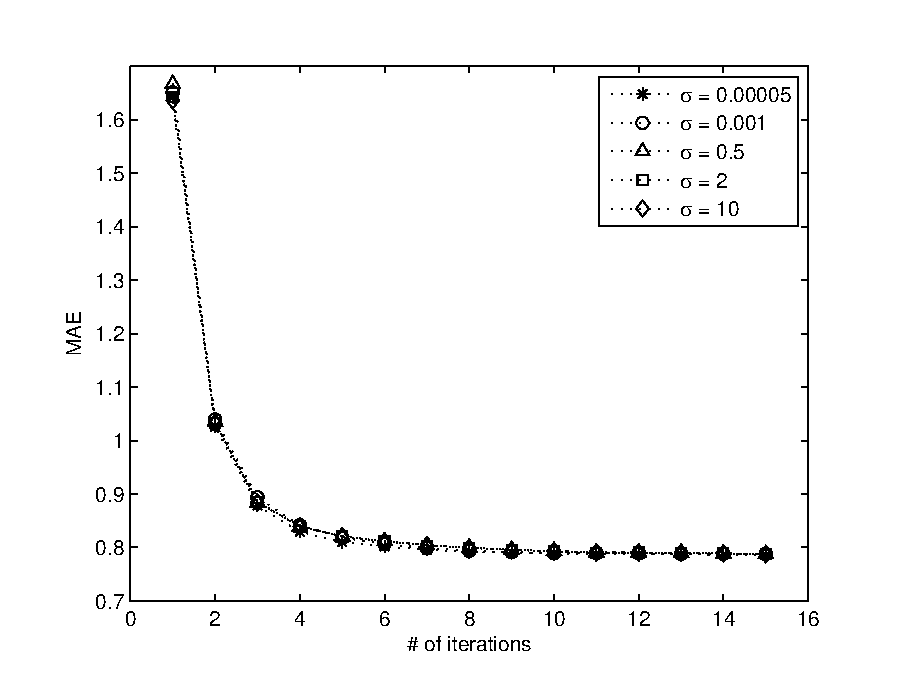
\includegraphics{3dimensions.eps}
\caption{Comparação de diferentes $\sigma$'s utilizando $k=3$}
\label{fig:3dimensions}
\end{figure}

Na figura \ref{fig:5dimensions}, onde $k=5$, novamente temos desempenhos muito próximos, entretanto notamos que, nas primeiras 4 iterações, $\sigma=10$ é melhor, enquanto que, a partir da 8ª iteração, $\sigma=0,00005$ é melhor. Já na figura \ref{fig:10dimensions}, onde $k=10$, $\sigma=10$ é claramente melhor. Por fim, quando tomamos $k=50$, na figura \ref{fig:50dimensions}, temos novamente o melhor resultado com $\sigma=0,00005$.

\begin{figure}[ht]
\centering
\includegraphics{5dimensions.eps}
\caption{Comparação de diferentes $\sigma$'s utilizando $k=5$}
\label{fig:5dimensions}
\end{figure}

\begin{figure}[ht]
\centering
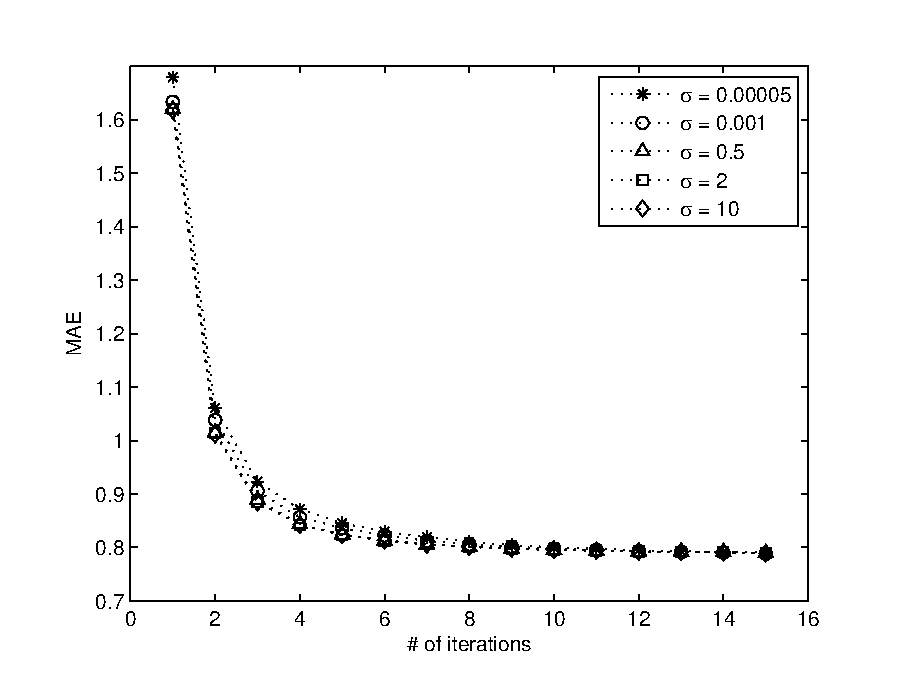
\includegraphics{10dimensions.eps}
\caption{Comparação de diferentes $\sigma$'s utilizando $k=10$}
\label{fig:10dimensions}
\end{figure}

\begin{figure}[ht]
\centering
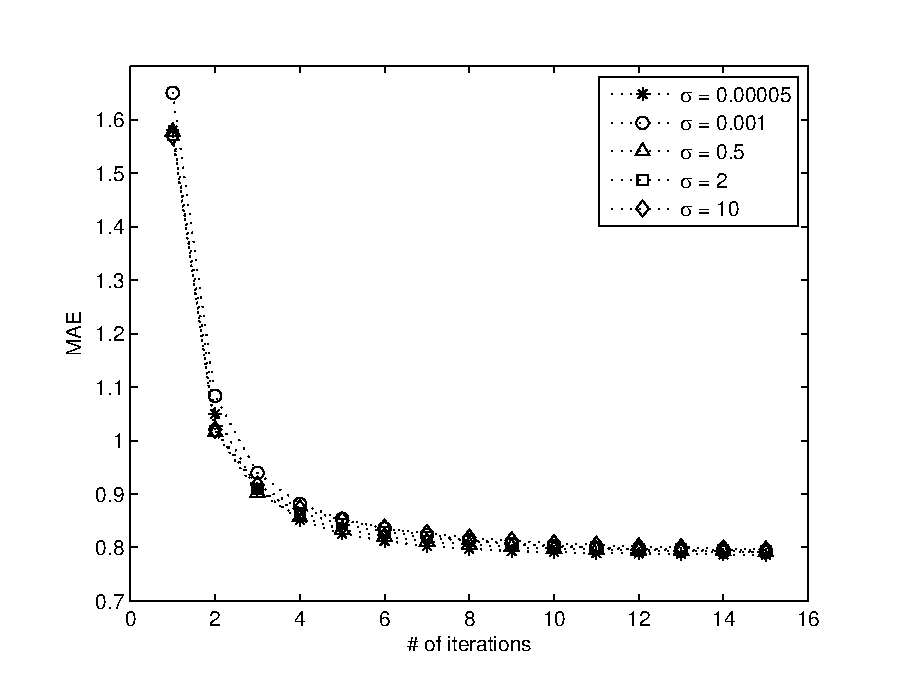
\includegraphics{50dimensions.eps}
\caption{Comparação de diferentes $\sigma$'s utilizando $k=50$}
\label{fig:50dimensions}
\end{figure}

Dado um valor para $k$, podemos concluir que as variações de desempenho percebidas, ao se mudar o parâmetro $\sigma$, são mínimas. Contudo, a fim de visualizarmos as variações de desempenho resultantes das mudanças em $k$, apresentamos na figura \ref{fig:final} o desempenho da \textit{Estratégia Livre de Viés}, para cada valor de $k$ testado, com seu respectivo melhor valor de $\sigma$. Como é possível observar, o melhor resultado ocorre com $k=2$ e $\sigma=0,00005$ e foram esses os parâmetros escolhidos para a \textit{Estratégia Livre de Viés} que será comparada com as demais no capitulo \ref{cap:resultados}.

\begin{figure}[ht]
\centering
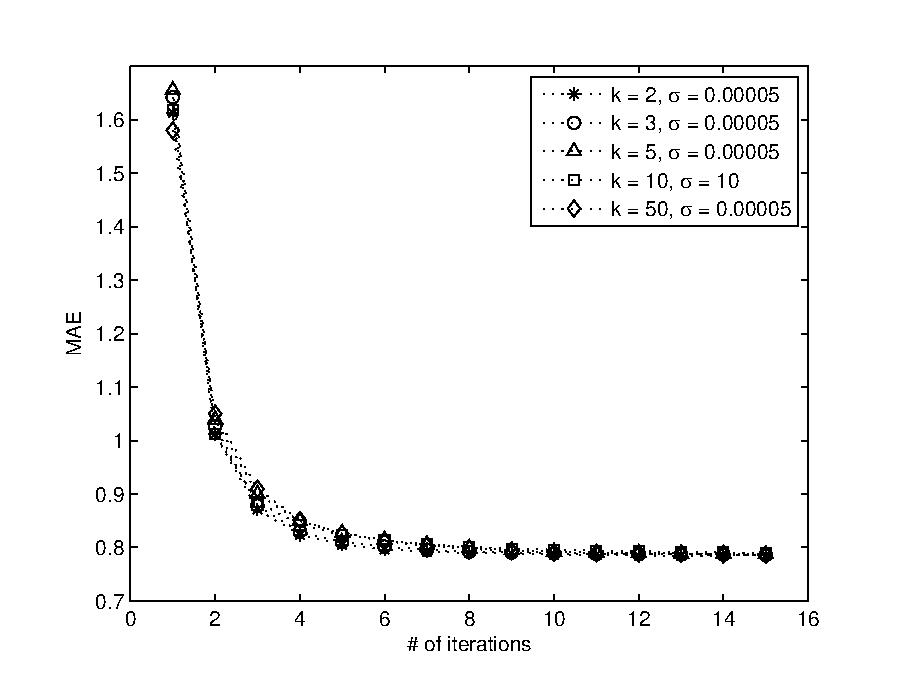
\includegraphics{final.eps}
\caption{Comparação de diferentes $k$'s com seus melhores $\sigma$'s}
\label{fig:final}
\end{figure}













  \chapter{Resultados}
\label{cap:resultados}

Antes de apresentarmos propriamente os resultados, faz-se necessário esclarecer o leitor sobre a maneira como os mesmos foram organizados. Em nossos experimentos, assim com em \citep{Elahi:2014:ALS:2542182.2542195}, um grande numero de estratégias, 17 no total, foram comparadas em termos de acurácia global do modelo (MAE). Visualizar os resultados de todas as estratégias ao mesmo tempo, ou seja, em um mesmo gráfico, acaba sendo improdutivo devido a grande quantidade de informação apresentada de uma só vez. Logo, optamos por dividir as estratégia em famílias e subdividir estas famílias em grupos, a fim de podermos analisar com melhor exatidão o desempenho de cada estratégia. Aliás, uma das críticas passíveis de ser feita a \citep{Elahi:2014:ALS:2542182.2542195} é o fato de que, ao mostrar todas as estratégias ao mesmo tempo, os gráficos acabam por ficar confusos, tolhendo o poder de analise.

\section{Organização}

Em linhas gerais, as estratégias foram divididas em 3 famílias: \textit{Entropia}, \textit{Variância} e \textit{Modelo}. Conforme o nome indica, a família \textit{Entropia} é constituída das estratégias que fazem uso da entropia das preferências. Ao todo, 7 estratégias pertencem à esta família, o que ainda é muita informação para ser analisada de maneira detalhada. Decidimos então por subdividir esta família em 4 grupos: \textit{Entropia Pura}; \textit{Logaritmo da Popularidade e Entropia}; \textit{Média Harmônica da Popularidade e Entropia}; e \textit{Ganho de Informação}.  

As estratégia foram divididas em grupos de acordo com suas características, assim, ao primeiro grupo pertencem as estratégias \textit{entropy} e \textit{entropy0}; ao segundo grupo pertencem as estratégias \textit{log(pop)*ent} e \textit{log(pop)*ent0}; ao terceiro grupo pertencem as estratégias \textit{helf} e \textit{helf0}; e, por fim, \textit{igcn} constitui sozinha o quarto grupo. 

A família \textit{Variância}, por sua vez, é constituída pelas estratégias que se baseiam na variância das preferências, i.e., \textit{variance}, \textit{log(pop)*var} e \textit{sqrt(pop)*var}. Por serem apenas 3 estratégias, não há necessidade de subdividi-las em grupos, posto que a apresentação das 3 em um mesmo gráfico não gera grandes dificuldades de analise.

Por fim, a família \textit{Modelo} agrega as estratégias que se baseiam no modelo, ou seja, no próprio algoritmo de recomendação. Decidimos por subdividi-las em dois grupos para facilitar a analise dos resultados. Estes foram formados de acordo com o desempenho das mesmas, assim, o primeiro, \textit{Pior que random}, é formado pelas estratégias \textit{bin pred} e \textit{high pred}. Já o segundo, \textit{Melhor que random}, é formado por \textit{low pred} e \textit{high low pred}.

Cada grupo será visualizado em conjunto com as estratégias de referência \textit{random} e \textit{popularity}. A avaliação de cada estratégia pode ser inferida de acordo com seu comportamento em relação a estas.

\section{Avaliação} 

Estamos avaliando cada estratégia no que diz respeito ao erro global do SR, i.e., o MAE. Obviamente quanto menor o valor do MAE, melhor é a estratégia. Contudo, estratégias de AA não são avaliadas em relação a um valor pontual de erro, e sim em relação ao decaimento dos erros pontuais, também conhecido como \textit{comportamento} da estratégia. Portanto, quanto mais acentuado, ou hiperbólico, for o decaimento do MAE, melhor é a estratégia.

Há duas estratégias clássicas que servirão de parâmetro para as outras, são elas \textit{random} e \textit{popularity}. A primeira, como veremos, possui um decaimento abrupto e bem acentuado, enquanto que a segunda possui um decaimento estável e pouco acentuado. Existem basicamente 3 áreas de desempenho para uma estratégia, ela pode ser pior que \textit{popularity}, i.e., seu comportamento se encontra acima da curva dada por esta; entre \textit{popularity} e \textit{random}, i.e., seu comportamento se encontra entre essas duas curvas; e melhor que \textit{random}, o que significa que seu comportamento se encontra abaixo desta curva, o melhor dos casos.

Ao fim, todas as estratégias atingem o mesmo valor de erro, visto que irão inserir todas as avaliações de $X$ em $K$ e, portanto, não importa qual estratégia usarmos, sempre atingiremos o limite inferior do nosso modelo. Em outras palavras, todas as possíveis estratégias irão convergir para o mesmo limiar definido apenas pelo modelo empregado. A este fenômeno, damos o nome de \textit{convergência} dos comportamentos.   

\section{Convergência}
 
Em termos práticos, a única diferença que existe entre os experimentos voltados para incentivos e os experimentos voltados para AF é o fato que, no caso de incentivos, o usuário sempre responde com as avaliações solicitadas. Isto não pode ser assumido como verdade no caso do AF, pois é possível que o usuário desconheça alguns dos itens solicitados, ou até mesmo todos. Quando tratamos de incentivos, é muito mais plausível assumir que o usuário consiguirá avaliar todos os itens solicitados, posto que são itens que ele já comprou e que haverá uma forma de ``recompensa'' se ele os avaliar.

Com isso, podemos esperar uma convergência mais rápida do MAE para o limiar do modelo. Vemos que isto se verifica em nossos resultados, uma vez que as estratégias parecem convergir a partir da 30ª iteração, em contrate com \citep{Elahi:2014:ALS:2542182.2542195}, onde a convergência se dá apenas por volta da 80ª iteração.

\section{Diferenças em relação a outros trabalhos}

Ainda em relação a \citep{Elahi:2014:ALS:2542182.2542195}, apesar de nossos experimentos serem semelhantes, esta suposição de que os usuários sempre colaboram avaliando todos os itens soliciados afeta significativamente nossos resultados em comparação com os de \citep{Elahi:2014:ALS:2542182.2542195}. As diferenças não aparecem apenas na questão da convergência, mas no comportamento das estratégias. Por exemplo, \citep{Elahi:2014:ALS:2542182.2542195} faz distinção entre estratégias \textit{monótonas} e \textit{não-monótonas}, enquanto que, em nossos resultados, nenhuma estratégia apresenta comportamento não-monótono.

Assim, embora os experimentos sejam muito parecidos, esta simples diferença torna os resultados difíceis de se comparar diretamente. Claro que o paralelo com \citep{Elahi:2014:ALS:2542182.2542195} foi realizado e, em alguns casos, houve forte correspondência entre os resultados. Porém, é importante o leitor ter em mente que as estratégias podem apresentar um comportamento diferente devido a estrutura do experimento em si, que é semelhante, mas não idêntica.

Outro trabalho que também nos serviu de inspiração e de balizamento foi \citep{Rashid:2008:LPN:1540276.1540302}. Várias das estratégias utilizadas em nossos experimentos foram extraídas de \citep{Rashid:2008:LPN:1540276.1540302} que, além de serem aplicadas diretamente, serviram de base para a criação de estratégias compostas. Todavia, há enormes diferenças entre nosso experimento e o descrito em \citep{Rashid:2008:LPN:1540276.1540302} que não derivam apenas do fato de \citep{Rashid:2008:LPN:1540276.1540302}, assim como \citep{Elahi:2014:ALS:2542182.2542195}, ser voltado para AF.

Primeiramente, \citep{Rashid:2008:LPN:1540276.1540302} procura elicitar as notas apenas dos usuários que avaliaram 80 itens ou mais, ignorando o resto. Além disso, o processo de elicitação é realizado em apenas uma iteração, buscando-se elicitar o maior número de itens possível de cada usuário ($N\geq75$). Por último, a avaliação das estratégias é realizada considerando somente as notas fornecidas pelo mesmo usuário na base de teste. Ou seja, \citep{Rashid:2008:LPN:1540276.1540302} compara o desempenho das estratégias com base nos usuários individuais e não no SR por completo.

Todas essas diferenças tornam a comparação de nossos resultados com os de \citep{Rashid:2008:LPN:1540276.1540302} muito difícil. Contudo, há casos onde os comportamentos das estratégias são semelhantes o que indica que, apesar das diferenças entre os experimentos, há uma forte sintonia entre os trabalhos.

\section{Entropia} 

\subsection{Entropia Pura}

As figuras \ref{fig:entropia-pura-movielens} e \ref{fig:entropia-pura-netflix} apresentam os comportamentos das estratégias \textit{entropy} e \textit{entropy0} nas bases \textit{MovieLens} e \textit{Netflix}, respectivamente. Em linhas gerais, podemos dizer que o comportamento de tais estratégias foi praticamente idêntico ao comportamento de \textit{popularity}, uma vez que as curvas de ambas parecem se sobrepor a esta última. No entanto, nas primeiras iterações, sobretudo na figura \ref{fig:entropia-pura-movielens}, \textit{entropy} parece ter um desempenho pior que \textit{popularity}, estando ligeiramente acima desta. 

Isto pode ser explicado pela própria diferença entre as estratégias. Enquanto \textit{entropy} busca solicitar os itens olhando apenas o valor de entropia dos mesmos, \textit{entropy0} procura levar em consideração também a impopularidade dos itens, adicionando no cálculo da entropia as preferências com valor zero. Pode-se dizer então que \textit{entropy0} leva em consideração a popularidade do item na medida em que considera a impopularidade do mesmo.

A deficiência da entropia pura foi comentada em detalhes em \citep{Rashid:2008:LPN:1540276.1540302}. Segundo este trabalho, calcular a entropia sem levar em consideração a popularidade do item pode ser enganoso, visto que itens que receberam poucas preferências podem possuir valores de entropia muito altos.

Infelizmente \citep{Elahi:2014:ALS:2542182.2542195} não apresenta resultados para estas estratégias. Todavia, devido ao desempenho ruim de ambas, concluímos que a heurística que as norteia resulta na construção de conjuntos de treinamento enviesados. Na prática, ao tentar reduzir a incerteza através da entropia, estamos adicionando no conjunto de treinamento apenas os itens mais controversos (os mais difíceis de se prever) e deixando de lado aqueles onde há maior consenso entre os usuários (os mais fáceis de se prever). A controvérsia dos itens acaba por se refletir na acurácia do modelo, que fica mais duvidoso e menos preciso ao calcular previsões.

\begin{figure}[ht]
\centering
\includegraphics{ml_ent_ent0.eps}
\caption{Avaliação do grupo \textit{Entropia Pura} na base \textit{MovieLens}}
\label{fig:entropia-pura-movielens}
\end{figure}

\begin{figure}[ht]
\centering
\includegraphics{nf_ent_ent0.eps}
\caption{Avaliação do grupo \textit{Entropia Pura} na base \textit{Netflix}}
\label{fig:entropia-pura-netflix}
\end{figure}

\subsection{Logaritmo da Popularidade e Entropia}

Do mesmo modo, as figuras \ref{fig:logpop-entropia-movielens} e \ref{fig:logpop-entropia-netflix} correspondem ao emprego de \textit{log(pop)*ent} e \textit{log(pop)*ent0} nas bases \textit{MovieLens} e \textit{Netflix}, respectivamente. Como é possível observar, ambas possuem comportamento muito similar a \textit{popularity}, entretanto havia indícios para suspeitarmos disso, uma vez que conhecemos os resultados do grupo \textit{Entropia Pura}.

Primeiramente, ambas estratégias estão baseadas no valor de popularidade, que representa o número de avaliações que o filme recebeu. Desta forma, tal valor, ainda que amenizado por uma função logarítmica, exerce forte influência sobre o comportamento da estratégia. Em segundo lugar, o outro componente que as compõe é o valor da entropia, dado pelas estratégias \textit{entropy} e \textit{entropy0}. É sabido que essas duas estratégias também não obtiveram comportamento muito destoante de \textit{popularity}. Logo, era esperado que tanto \textit{log(pop)*ent} como \textit{log(pop)*ent0} apresentassem comportamentos semelhantes à \textit{popularity}.

Fazendo uma analogia com o mercado de ações, podemos dizer que \textit{log(pop)*ent} está ``indexada'' por \textit{popularity} e \textit{entropy}, enquanto que \textit{log(pop)*ent0} está ``indexada'' por \textit{popularity} e \textit{entropy0}. Ou seja, assim como um fundo de investimento que está indexado por um determinado ativo (composto majoritariamente por este ativo) não apresentará rendimentos que destoam significativamente do rendimento deste ativo, da mesma maneira, o comportamento de tais estratégias não será muito distante do comportamento das suas estratégias ``índices''.

Em \citep{Elahi:2014:ALS:2542182.2542195} são apresentados apenas as estratégias \textit{log(pop)*ent} e \textit{popularity} e pode-se verificar que os comportamentos de ambas seguem bem próximos, o que confirma nossa analogia. 

\begin{figure}[ht]
\centering
\includegraphics{ml_logpopent_logpop_ent0.eps}
\caption{Avaliação do grupo \textit{Logaritmo da Popularidade e Entropia} na base \textit{MovieLens}}
\label{fig:logpop-entropia-movielens}
\end{figure}

\begin{figure}[ht]
\centering
\includegraphics{nf_logpopent_logpopent0.eps}
\caption{Avaliação do grupo \textit{Logaritmo da Popularidade e Entropia} na base \textit{Netflix}}
\label{fig:logpop-entropia-netflix}
\end{figure}

\subsection{Média Harmônica da Popularidade e Entropia}

Novamente, pode-se observar a atração que as estratégias índices aplicam sobre suas indexadas. Vemos através das figuras \ref{fig:helf-movielens} e \ref{fig:helf-netflix} que \textit{helf} e \textit{helf0} recaem sobre \textit{popularity}. 

Este resultado, juntamente com o anterior, nos informa que tanto combinações simples (e.g., função logarítmica) como combinações complexas (e.g., média harmônica) não suprimem a atração que as estratégias compostas sofrem daquelas que as compõem. Concluímos então que a utilização de estratégias compostas, ou indexadas, não trará ganhos significativos quando as estratégias simples, as que lhes servem como índices, não possuem um bom comportamento elas mesmas.

Apesar de \citep{Elahi:2014:ALS:2542182.2542195} não fazer uso de \textit{helf} nem de \textit{helf0} em seus experimentos, os autores em \citep{Rashid:2008:LPN:1540276.1540302} apresentam os resultados que obtiveram com \textit{helf}. Conforme deduzido aqui, eles seguem bem próximos ao comportamento de \textit{popularity}. 

\begin{figure}[ht]
\centering
\includegraphics{ml_helf_helf0.eps}
\caption{Avaliação do grupo \textit{Média Harmônica da Popularidade e Entropia} na base \textit{MovieLens}}
\label{fig:helf-movielens}
\end{figure}

\begin{figure}[ht]
\centering
\includegraphics{nf_helf_helf0.eps}
\caption{Avaliação do grupo \textit{Média Harmônica da Popularidade e Entropia} na base \textit{Netflix}}
\label{fig:helf-netflix}
\end{figure}

\subsection{Ganho de Informação}

Dentre as estratégias da família \textit{Entropia}, \textit{igcn} parece ter obtido o melhor comportamento, conforme as figuras \ref{fig:igcn-movielens} e \ref{fig:igcn-netflix} indicam. Entretanto, mesmo sendo a melhor estratégia da família \textit{Entropia}, ela ainda fica muito aquém do desejado, que seria ultrapassar a estratégia \textit{random}.

Apesar de estar inserida nesta família, a \textit{igcn} não se baseia na entropia das preferências, mas sim na entropia dos usuários. Segundo \citep{Rashid:2008:LPN:1540276.1540302}, trabalho que propôs a estratégia, os usuários são divididos em grupos, chamados de \textit{clusters}, de acordo com suas disposições no espaço dado pela decomposição SVD. Os itens solicitados são aqueles que, se avaliados, reduzirão a incerteza associada a distribuição dos usuários em \textit{clusters}, i.e., trarão a maior redução na entropia da distribuição dos usuários.

Aqui, como no caso já comentado da entropia pura, há uma heurística subjacente à estratégia que parece introduzir viés no conjunto de treinamento. Buscar os itens com maior potencial para ``organizar'' os usuários, dentro de um espaço vetorial construído com base nas avaliações, não implica necessariamente em redução do erro do modelo. Afinal, é possível que o estado natural dos dados, incluindo as disposições dos usuários em tal espaço, seja um estado de desordem. Ao solicitar os itens que trarão uma maior organização, estamos induzindo uma ordem que é estranha aos dados e, consequentemente, podemos estar enviesando o conjunto de treinamento.

Somente \citep{Rashid:2008:LPN:1540276.1540302} apresenta resultados para \textit{igcn}, porém, infelizmente, não há comparações com \textit{random}. Todavia, faz-se comparações com \textit{helf}, \textit{entropy0} e \textit{popularity}, as quais se mostraram inferiores à \textit{igcn}, similar ao que foi verificado em nossos experimentos.

\begin{figure}[ht]
\centering
\includegraphics{ml_igcn.eps}
\caption{Avaliação do grupo \textit{Ganho de Informação} na base \textit{MovieLens}}
\label{fig:igcn-movielens}
\end{figure}

\begin{figure}[ht]
\centering
\includegraphics{nf_igcn.eps}
\caption{Avaliação do grupo \textit{Ganho de Informação} na base \textit{Netflix}}
\label{fig:igcn-netflix}
\end{figure}

\section{Variância}

Na família \textit{Variância}, como há apenas três estratégias, decidimos por não dividir em grupos e apresentá-las todas de uma só vez. Os resultados podem ser vistos nas figuras \ref{fig:variance-movielens} e \ref{fig:variance-netflix}, paras as bases \textit{Movielens} e \textit{Netflix}, respectivamente.

Vemos que a estratégias \textit{variance} apresenta uma ligeira vantagem sobre as demais, sobretudo na figura \ref{fig:variance-movielens}, nas primeiras 10 iterações. Contudo, seu comportamento passa logo a seguir o de \textit{popularity}, o que aponta para a presença de viés em $K$. Novamente, como no caso da entropia, tentar minimizar a incerteza dos itens através da variância, acarreta na construção de um conjunto de treinamento dominado pelos itens mais controversos. Tais itens são justamente os mais difíceis de se prever avaliações e, portanto, o modelo tem grande dificuldade em capturar o padrão que determina as avaliações dadas pelos usuários.  

As estratégias compostas utilizando \textit{variance} e \textit{popularity} caem no mesmo inconveniente das estratégias compostas que fazem uso de \textit{entropy} (ou \textit{entropy0}) e \textit{popularity}, ou seja, acabam por serem atraídas para o comportamento de \textit{popularity}. O que explica a semelhança de comportamento tanto de \textit{log(pop)*var} de \textit{sqrt(pop)*var} com \textit{popularity}.

\begin{figure}[ht]
\centering
\includegraphics{ml_variance_family.eps}
\caption{Avaliação da família \textit{Variância} na base \textit{MovieLens}}
\label{fig:variance-movielens}
\end{figure}

\begin{figure}[ht]
\centering
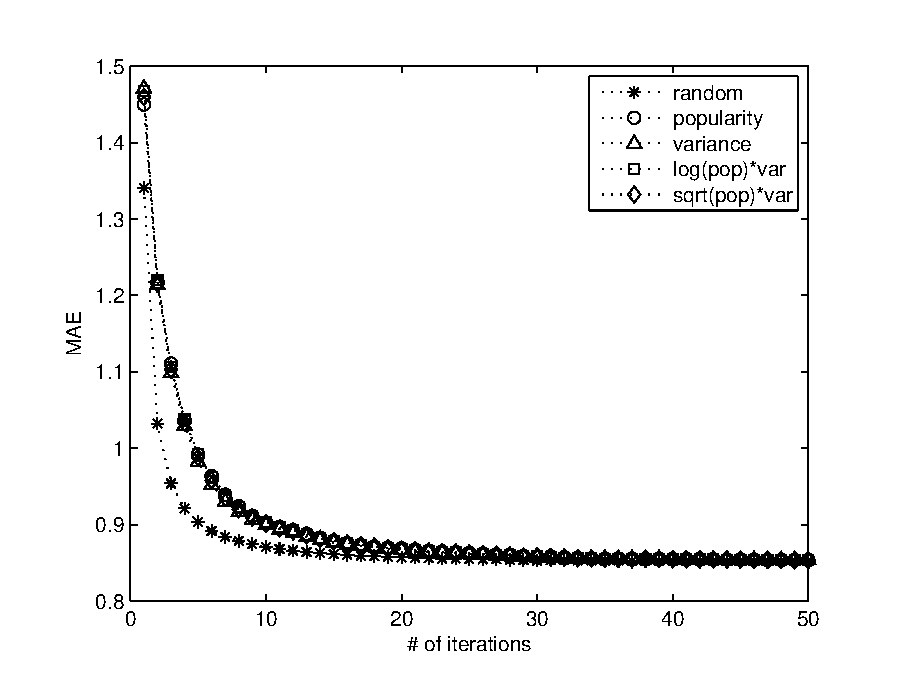
\includegraphics{nf_variance_family.eps}
\caption{Avaliação da família \textit{Variância} na base \textit{Netflix}}
\label{fig:variance-netflix}
\end{figure}

\section{Modelo}

Dentre as estratégias da família \textit{Modelo}, duas delas obtiveram desempenho pior que a estratégia \textit{random}, enquanto que as outras duas foram melhores. Aliás, deve-se mencionar que foram as únicas de todo nosso experimento que conseguiram tal feitio, com exceção da \textit{Estratégia Livre de Viés}. Cabe à nós então analisarmos o porquê deste comportamento inusitado, tendo sempre em mente a heurística por trás de cada estratégia.

\subsection{Pior que \textit{random}}

Começaremos por analisar as estratégias que obtiveram desempenho pior que \textit{random}, isto é, \textit{high pred} e \textit{bin pred}, exibidas nas figuras \ref{fig:worst-random-movielens} e \ref{fig:worst-random-netflix}. Observamos que ambas, até a 10ª iteração, apresentam desempenho ligeiramente superior à \textit{popularity}, convergindo mais tarde para o comportamento desta.

É importante levar em consideração que ambas as bases contêm preferências em forma de números inteiros, variando de 1 a 5. Das 100 mil avaliações presentes na base \textit{MovieLens}, cerca de 6\% das notas possuem valor igual a 1; 12\% igual a 2; 27\% igual a 3; 34\% igual a 4; e 21\% igual 5. Na base \textit{Netflix}, por sua vez, das 100 mil avaliações, cerca de 8\% possuem valor igual a 1; 14\% igual a 2; 35\% igual a 3; 27\% igual a 4; e 16\% igual a 5.

Se considerarmos as notas 1 e 2 como avaliações ``baixas'', e as notas 3, 4 e 5 como avaliações ``altas'', verificamos que \textit{MovieLens} e \textit{Netflix} possuem 82\% e 78\% das notas como sendo altas, respectivamente. Esta característica pode elucidar muito a respeito do desempenho que tais estratégias tiveram nessas bases.

A estratégia \textit{high pred} busca solicitar os itens que receberam as melhores previsões do modelo, ou seja, itens cujas previsões apontam para preferências altas. Desta maneira, ela insere no conjunto de treinamento $K$ sempre preferências altas, agravando o desequilíbrio natural que existe entre as preferências e tornando o conjunto ainda mais desbalanceado. Como o modelo é treinado com as preferências em $K$, este desequilíbrio transfere-se para a acurácia do mesmo, que acaba por ficar mais preciso em prever preferências altas do que baixas.

Por sua vez, \textit{bin pred} procura inserir em $K$ os itens cujas previsões apontam para alguma preferência, seja ela baixa ou alta. Em outras palavras, \textit{bin pred} solicita os itens cujas previsões indicam que os mesmos serão ``consumidos''. Esta abordagem não faz distinção entre as preferências, reduzindo-as a simples informações binárias. Com isso, acabamos simplesmente mantendo o desequilíbrio natural das preferências, visto que, ao contrário do caso de \textit{high pred}, não temos nenhuma ideia de como o usuário avaliará os itens solicitados.

Ambas as estratégias apresentam desempenho ruim em \citep{Elahi:2014:ALS:2542182.2542195}, ou seja, pior que \textit{random}. Contudo, no referido trabalho, \textit{bin pred} é nitidamente melhor que \textit{high pred}, o que não ficou claro em nossos experimentos. Na medida em que solicita apenas os itens de previsão alta, \textit{high pred} reforça o desequilíbrio entre as preferências em $K$, agravando a disparidade entre as previsões. Como \textit{bin pred} não sabe qual foi o valor efetivo da preferência prevista, o desequilíbrio em $K$ apenas se mantem com os itens solicitados. Por exemplo, mesmo que haja itens com previsão alta, é possível que \textit{bin pred} solicite itens com previsão baixa, o que não seria possível em \textit{high pred}.  

\begin{figure}[ht]
\centering
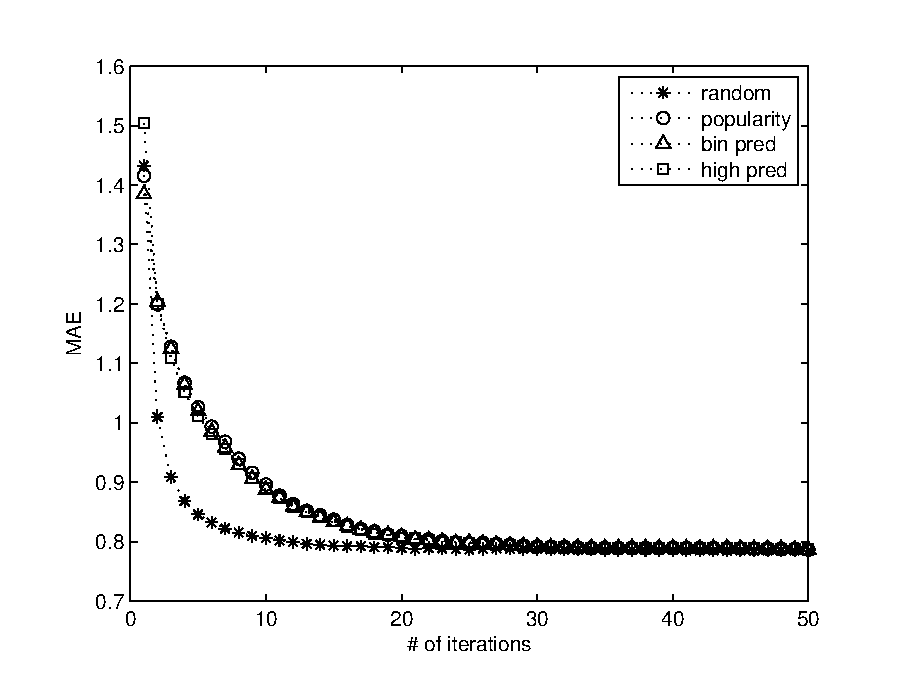
\includegraphics{ml_bin_high.eps}
\caption{Avaliação do grupo \textit{Pior que random} na base \textit{MovieLens}}
\label{fig:worst-random-movielens}
\end{figure}

\begin{figure}[ht]
\centering
\includegraphics{nf_bin_high.eps}
\caption{Avaliação do grupo \textit{Pior que random} na base \textit{Netflix}}
\label{fig:worst-random-netflix}
\end{figure}

\subsection{Melhor que \textit{random}}
\label{sec:melhor-random}

As únicas estratégias que obtiveram desempenho melhor que \textit{random}, com exceção da \textit{Estratégia Livre de Viés}, foram \textit{low pred} e \textit{high-low pred}, conforme pode ser observado nas figuras \ref{fig:better-random-movielens} e \ref{fig:better-random-netflix}.

Ao contrário de \textit{high pred}, \textit{low pred} busca solicitar os itens cujas previsões apontam para preferências baixas. Uma vez que há uma carência natural por tais preferências, ao solicitá-las, esta estratégia introduz em $K$ justamente as preferências faltantes, amenizando o desequilíbrio entre preferências baixas e altas. O conjunto de treinamento acaba ficando mais equilibrado e, consequentemente, a acurácia do modelo fica mais balanceada, capaz de fazer previsões mais precisas para todos os tipos de preferência. 

Ou seja, a estratégia \textit{low pred} se beneficia da carência natural de preferências baixas. A heurística que a norteia, solicitar os itens com previsões baixas, mostrou-se eficaz visto que as bases utilizadas em nossos experimentos carecem de tais preferências. Caso as características das bases fossem outras ou se modificassem com o tempo, o desempenho da estratégia poderia ser diferente. Em outras palavras, o simples fato de que a estratégia obteve um bom desempenho não significa que ela não introduz viés no conjunto de treinamento. Pelo contrário, a própria concepção da estratégia implica na construção de um conjunto de treinamento enviesado, porém, neste caso, o viés nos foi útil.

Da mesma forma, \textit{high-low pred} assume que é preferível solicitar itens cujas previsões se distanciam do valor médio de preferência. Em ambas as bases, as avaliações podem possuir valores inteiros de 1 a 5, sendo o valor médio 3. Logo, \textit{high-low pred} procura solicitar itens cuja previsão é igual a 1 ou 5 (valores mais distantes do valor médio). Se definirmos as notas 1 e 5 como sendo avaliações ``extremas'' e as notas 2, 3, e 4 como avaliações ``medianas'', constatamos que 73\% das avaliações em \textit{MovieLens} são medianas, enquanto que, em \textit{Netflix}, este percentual é de 76\%.

Ou seja, a distinção entre avaliações baixas e altas esconde um pouco o verdadeiro desequilíbrio entre as preferências. Na verdade, as notas 3 e 4 compõem a grande maioria das avaliações nas duas bases, sendo 61\% das avaliações em \textit{MovieLens} e 62\% em \textit{Netflix}. Assim como \textit{low pred}, ao solicitar os itens cujas previsões apontam para preferências extremas, \textit{high-low pred} ameniza o desequilíbrio natural que existe nas bases e promove um treinamento mais balanceado do modelo. A heurística subjacente à estratégia acaba sendo, mais uma vez, útil, pois ataca justamente a desproporção entre as preferências. 

Em \citep{Elahi:2014:ALS:2542182.2542195}, tanto \textit{low pred} quanto \textit{high-low pred} apresentam desempenho pior que \textit{random} nas primeiras iterações, porém conseguem alcançar e superar esta estratégia. No entanto, \textit{high-low pred} mostrou-se melhor que \textit{low pred}, o que não ficou claro em nosso trabalho. Isto significa que a distinção entre preferências ``extremas'' e ``medianas'' representa melhor a realidade dos dados do que a distinção entre preferências ``baixas'' e ``altas''. 

%O bom desempenho de \textit{high-low pred}, por sua vez, pode ser explicado pelo mesmo argumento utilizado para justificar o desempenho das estratégias indexadas (e.g., \textit{helf}, \textit{log(pop)*ent0}, etc.). Isto é, como \textit{high-low pred} está indexada por \textit{low pred}, o comportamento da estratégia índice acaba por atrair o comportamento da indexada.
%O curioso de notar neste caso é que \textit{high-low pred} também está indexa por \textit{high pred}, que, por sua vez, não obteve um bom desempenho. Assim, temos motivos para supor que uma estratégia indexada por duas ou mais estratégias será atraída mais fortemente pela estratégia índice com melhor desempenho, contudo, maiores evidências se fazem necessárias para que possamos concluir de fato esta propriedade. Verificamos que \textit{low pred} e \textit{high-low pred} apresentam comportamentos semelhantes em \citep{Elahi:2014:ALS:2542182.2542195}, o que traz mais crédito à nossa análise.

\begin{figure}[ht]
\centering
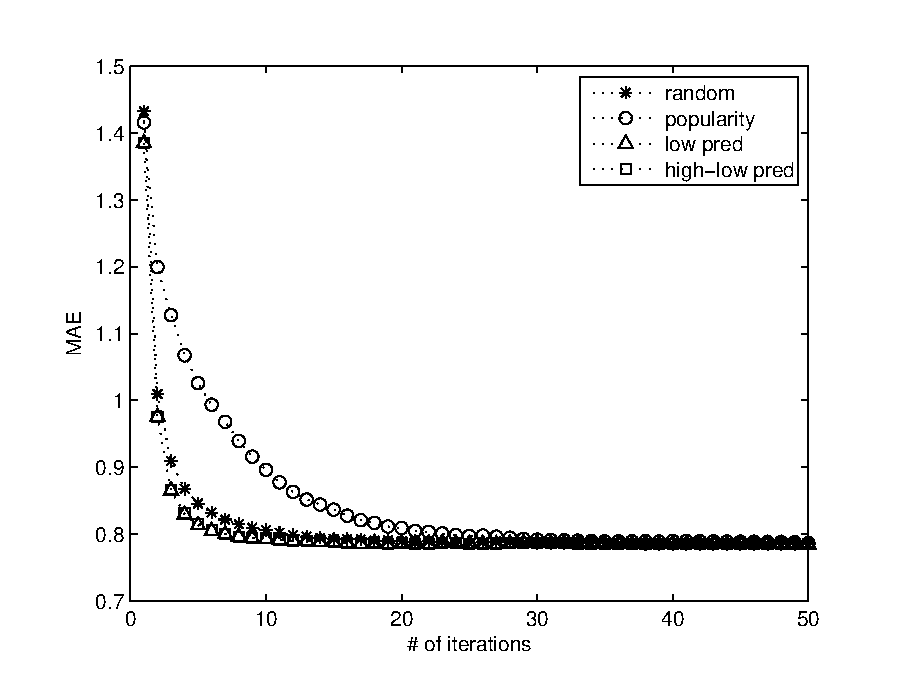
\includegraphics{ml_low_highlow.eps}
\caption{Avaliação do grupo \textit{Melhor que random} na base \textit{MovieLens}}
\label{fig:better-random-movielens}
\end{figure}

\begin{figure}[ht]
\centering
\includegraphics{nf_low_highlow.eps}
\caption{Avaliação do grupo \textit{Melhor que random} na base \textit{Netflix}}
\label{fig:better-random-netflix}
\end{figure}

\section{Estratégia Livre de Viés}

Iremos analisar nas próximas seções o comportamento da \textit{Estratégia Livre de Viés}, nomeada como \textit{unbiased} em nossos experimentos, comparando seu comportamento com as duas melhores estratégias até então: \textit{low pred} e \textit{high-low pred}. Além de uma análise global, visualizando todas as iterações, optamos também por realizar uma análise ampliada, com foco nas primeiras 15 primeiras iterações, onde é possível perceber mais nitidamente a superioridade de \textit{unbiased}.

\subsection{\textit{unbiased vs. low pred}}

As figuras \ref{fig:unbiased-lowpred-global-movielens} e \ref{fig:unbiased-lowpred-global-netflix} apresentam uma visão global, ou seja, uma visualização dos comportamentos de \textit{low pred} e \textit{unbiased} durante todas as iterações, nas bases \textit{MovieLens} e \textit{Netflix}, respectivamente. É possível verificar que, nas duas primeiras iterações, \textit{low pred} apresenta certa vantagem, entretanto, a partir da 3ª iteração, \textit{unbiased} parece alcançá-la e acompanhá-la até o final. Infelizmente, como o ganho de \textit{unbiased} é muito sutil, não conseguimos percebê-lo nesta escala.

Assim, decidimos por apresentar uma visão ampliada dos comportamentos de \textit{low pred} e \textit{unbiased}, até a 15ª iteração, de modo que seja possível visualizar com clareza a vantagem desta última. As figuras \ref{fig:unbiased-lowpred-focus-movielens} e \ref{fig:unbiased-lowpred-focus-netflix} exibem esta visão ampliada nas bases \textit{MovieLens} e \textit{Netflix}, respectivamente.

Vemos que \textit{unbiased} começa pior que \textit{low pred} em ambas as bases, porém, passadas algumas iterações, a primeira alcança a segunda e a supera. É interessante notar que, na base \textit{MovieLens}, \textit{unbiased} alcança \textit{low pred} já na 3ª iteração, enquanto que, em \textit{Netflix}, o empate só se dá por volta da 9ª iteração. Contudo, após o ponto de empate, em ambas as bases, pode-se observar que \textit{unbiased} toma a preeminência sobre a acurácia.

Um detalhe interessante é que esta preeminência de \textit{unbiased} é muito mais explícita na base \textit{MovieLens} do que na base \textit{Netflix}. Além do ponto de empate ocorrer mais cedo, o desvio padrão da acurácia, denotado pelas barras verticais, de \textit{unbiased} está abaixo do de \textit{low pred} em \textit{MovieLens} e eles não se sobrepõem. Isto significa que, mesmo no seu pior momento, o desempenho de \textit{unbiased} ainda é melhor do que o melhor momento de \textit{low pred}.

Embora este resultado nos remeta a conclusão de que \textit{unbiased} é efetivamente melhor que \textit{low pred}, é preciso lembrar que nossas conclusões devem se limitar ao dados em questão. Ou seja, apesar do comportamento de \textit{unbiased} ser nitidamente melhor que \textit{low pred}, na base \textit{MovieLens}, os resultados na base \textit{Netflix} já nos levam a uma conclusão diferente. Na média, o comportamento de \textit{unbiased} até foi superior ao de \textit{low pred} em \textit{Netflix}, no entanto, vemos que o desvio padrão das duas estratégias sobrepõem-se nesta base, o que indica que \textit{low pred}, em seus melhores momentos, pode superar \textit{unbiased}. 

Esta superioridade de \textit{unbiased} em \textit{MovieLens} pode ser explicada pelo fato de que a escolha dos parâmetros de \textit{unbiased} foi realizada com base apenas em \textit{MovieLens}. É possível que, utilizando parâmetros diferentes, possamos atingir resultados em \textit{Netflix} similares aos de \textit{MovieLens}. 

\begin{figure}[ht]
\centering
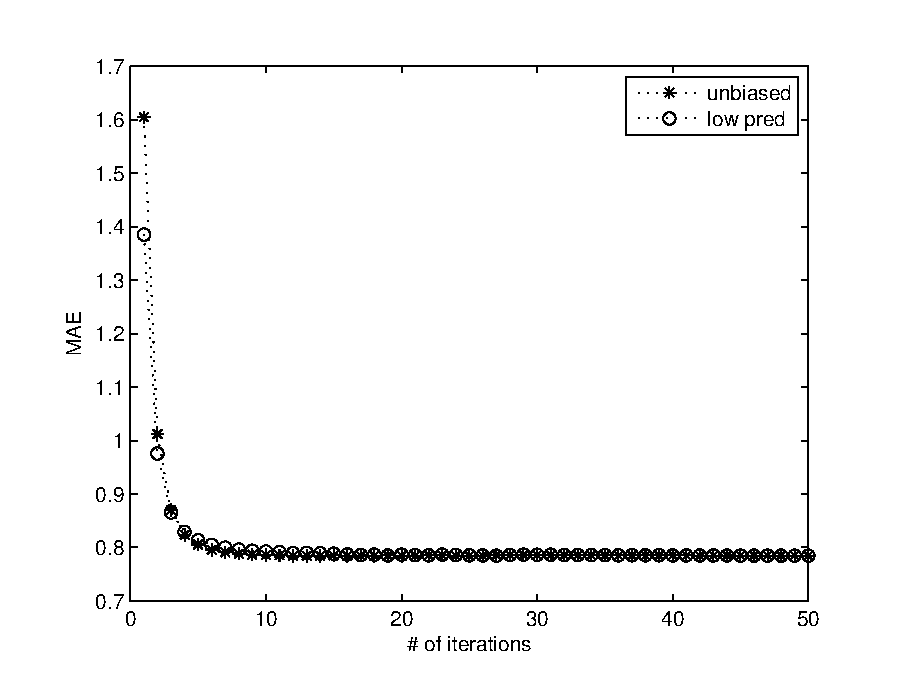
\includegraphics{ml_global_low_unbiased.eps}
\caption{Visão global de \textit{unbiased vs. low pred}  na base \textit{MovieLens}}
\label{fig:unbiased-lowpred-global-movielens}
\end{figure}

\begin{figure}[ht]
\centering
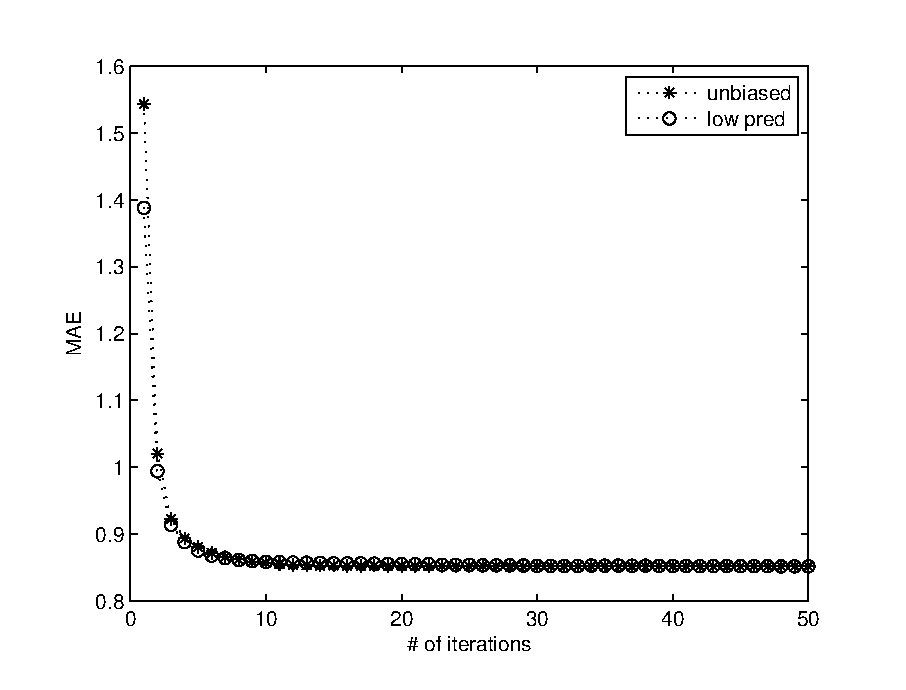
\includegraphics{nf_global_low_unbiased.eps}
\caption{Visão global de \textit{unbiased vs. low pred} na base \textit{Netflix}}
\label{fig:unbiased-lowpred-global-netflix}
\end{figure}

\begin{figure}[ht]
\centering
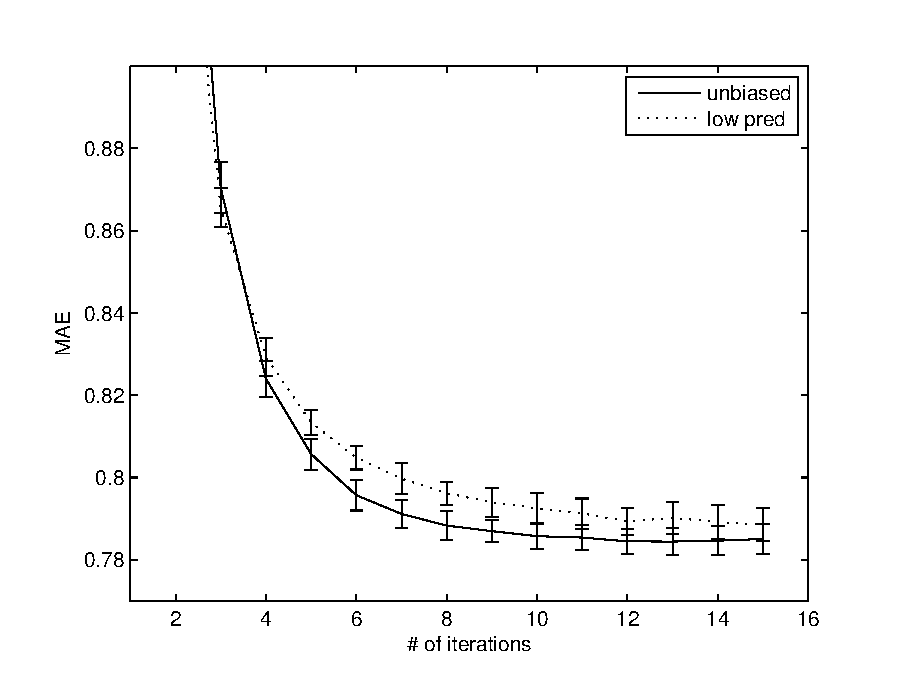
\includegraphics{ml_focus_low_unbiased.eps}
\caption{Visão ampliada de \textit{unbiased vs. low pred} na base \textit{MovieLens}}
\label{fig:unbiased-lowpred-focus-movielens}
\end{figure}

\begin{figure}[ht]
\centering
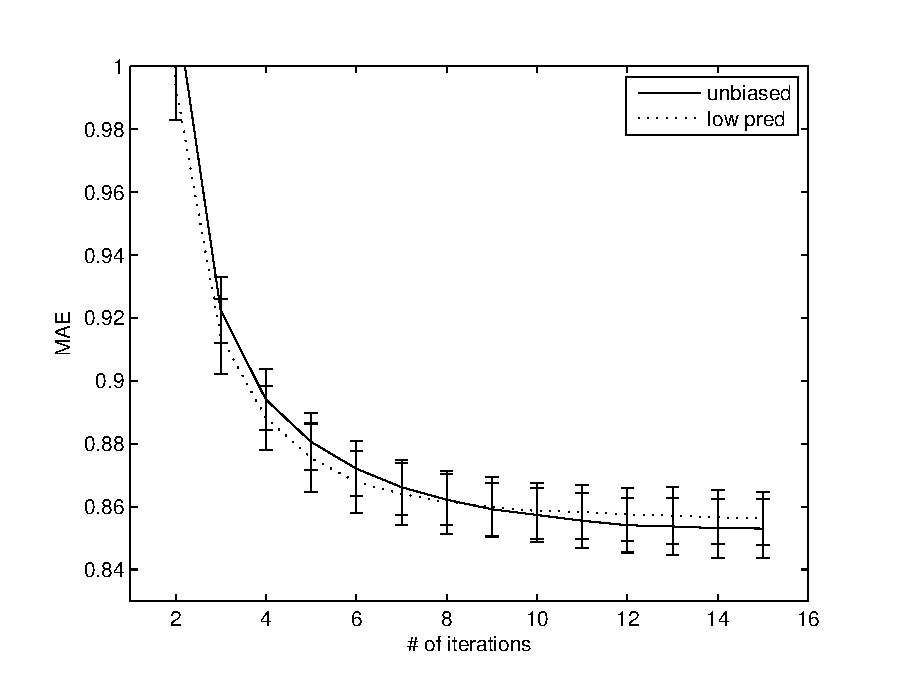
\includegraphics{nf_focus_low_unbiased.eps}
\caption{Visão ampliada de \textit{unbiased vs. low pred} na base \textit{Netflix}}
\label{fig:unbiased-lowpred-focus-netflix}
\end{figure}

\subsection{\textit{unbiased vs. high-low pred}}

Quando comparamos \textit{unbiased} com \textit{high-low pred} encontramos resultados muito parecidos com a comparação feita com \textit{low pred}. As figuras \ref{fig:unbiased-highlowpred-global-movielens} e \ref{fig:unbiased-highlowpred-global-netflix} exibem a visão global para as bases \textit{MovieLens} e \textit{Netflix}, respectivamente. Através delas, observa-se que, em ambas as bases, \textit{unbiased} começa com uma notória desvantagem frente a \textit{high-low pred}, porém, já na 3ª iteração, ambas parecem confluir para um mesmo valor e seguem assim até o final do experimento.

Na visão ampliada para as bases \textit{MovieLens} e \textit{Netflix}, obtida através das figuras \ref{fig:unbiased-highlowpred-focus-movielens} e \ref{fig:unbiased-highlowpred-focus-netflix}, respectivamente, vê-se que o ponto de empate de \textit{unbiased} e \textit{high-low pred}, em \textit{MovieLens}, se dá pela 3ª iteração, enquanto que, em \textit{Netflix}, este ponto se dá pela 9ª iteração. Além disso, a relação entre os desvios padrão também se mantem a mesma, já que em \textit{MovieLens} não há sobreposição e em \textit{Netflix} há.

De fato, não deveríamos esperar um resultado diferente para a comparação com \textit{high-low pred}. Tanto \textit{low pred} e \textit{high-low pred} se baseiam em heurísticas que procuram tornar o conjunto de treinamento mais balanceado. \textit{low pred} dá prioridade a itens com previsões 1 e 2 por serem avaliações ``baixas'', enquanto que \textit{high-low pred} também dá prioridade a itens com previsão 1 e 2 por serem ``extremas''. Assim, é esperado que haja uma enorme interseção dos itens solicitados por ambas as estratégias e, consequentemente, uma sintonia muito forte de seus comportamentos. Além disso, a questão dos parâmetros também influencia a obtenção do melhor resultado em \textit{MovieLens}.

\begin{figure}[ht]
\centering
\includegraphics{ml_global_highlow_unbiased.eps}
\caption{Visão global de \textit{unbiased vs. high-low pred}  na base \textit{MovieLens}}
\label{fig:unbiased-highlowpred-global-movielens}
\end{figure}

\begin{figure}[ht]
\centering
\includegraphics{nf_global_highlow_unbiased.eps}
\caption{Visão global de \textit{unbiased vs. high-low pred} na base \textit{Netflix}}
\label{fig:unbiased-highlowpred-global-netflix}
\end{figure}

\begin{figure}[ht]
\centering
\includegraphics{ml_focus_highlow_unbiased.eps}
\caption{Visão ampliada de \textit{unbiased vs. high-low pred} na base \textit{MovieLens}}
\label{fig:unbiased-highlowpred-focus-movielens}
\end{figure}

\begin{figure}[ht]
\centering
\includegraphics{nf_focus_highlow_unbiased.eps}
\caption{Visão ampliada de \textit{unbiased vs. high-low pred} na base \textit{Netflix}}
\label{fig:unbiased-highlowpred-focus-netflix}
\end{figure}
  \chapter{Conclusões e Trabalhos Futuros}
\label{cap:conclusao}

Há três resultados importantes em nossos experimentos que merecem atenção. O primeiro é o bom desempenho obtido por \textit{random} ou, olhando sob outro aspecto, o desempenho ruim obtido pela maioria das estratégias, com exceção de \textit{low pred} e \textit{high-low pred}. As heurísticas que formulam as estratégias ditam a maneira como os itens serão selecionados para inclusão no conjunto de treinamento. Por exemplo, \textit{entropy}, \textit{variance} e suas derivadas assumem que os melhores itens a serem incluídos no conjunto de treinamento são aqueles mais controversos; \textit{igcn} assume que os melhores itens são aqueles que melhor distribuem os usuários em \textit{clusters}; \textit{high pred} assume que o melhor conjunto de treinamento é aquele formado por itens com as maiores avaliações; enquanto que \textit{bin pred} assume que o melhor conjunto é aquele formado por itens com grande chance de serem consumidos.

Em todos esses casos, há uma suposição, ou heurística, que guia a seleção dos itens, gerando assim um conjunto formado por itens que satisfazem esta suposição e não necessariamente por aqueles que melhor representam a população de itens. Seria correto afirmar então que o emprego de estratégias de AA quase sempre acarreta em conjuntos de treinamento enviesados, o que, à primeira vista, pode parecer indesejado. No entanto, ter um conjunto de treinamento enviesado nem sempre é algo ruim. Nosso segundo resultado digno de ser destacado é o fato de que \textit{low pred} e \textit{high-low pred} obtiveram bons resultados mesmo formando conjuntos de treinamento enviesados. Ou seja, há casos onde um conjunto enviesado pode ser útil. 

Em nossos experimentos, como as preferências 3 e 4 excedem as demais, um conjunto equilibrado promoveu um bom desempenho do modelo, apesar de ser, tecnicamente, enviesado. Todavia, em situações reais muitas vezes não se conhece as características da base de dados, sem mencionar que as mesmas estão em constante mutação conforme a base cresce. Mesmo em um ambiente isolado e controlado como o nosso, foi necessário testar várias estratégias, baseadas em diversas heurísticas diferentes, para encontrarmos aquela que é adequada aos dados (apenas duas heurísticas se mostraram adequadas). Efetuar tal comparação em um sistema real seria muito complexo, sem contar que o resultado seria provisório dado o carácter volátil de um SR. Ou seja, os projetistas de SR necessitam de uma estratégia que possa ser utilizada em qualquer ocasião, sejam quais forem as características da base de dados e, de preferência, independentemente do modelo adotado.

Isto nos leva ao terceiro resultado que é o excelente desempenho obtido pela \textit{Estratégia Livre de Viés}. Tal estratégia assume que o melhor conjunto de treinamento é simplesmente aquele que melhor representa a população, ou seja, aquele onde não há viés. Nossos experimentos mostraram que a \textit{Estratégia Livre de Viés} de fato promove o bom desempenho do modelo, superando às demais. Embora ainda desejamos realizar mais testes, em outras bases, acreditamos ter encontrado uma excelente opção, dentre as diversas estratégias da literatura, que pode ser empregada em qualquer ocasião, sob quaisquer circunstâncias e com qualquer modelo de recomendação. Assim, a \textit{Estratégia Livre Viés} é uma ótima opção para um SR, visto que o risco relacionado à adoção de outra estratégia, cuja heurística pode não condizer com os dados, é alto.

Como trabalhos futuros, além de analisar o comportamento da \textit{Estratégia Livre de Viés} com bases maiores, pretendemos analisá-la sob situações reais. O problema de \textit{Elicitação de Preferências para fins de Incentivo} possui muitas nuances que só podem ser examinadas em um ambiente \textit{online}. Para tal, desejamos utilizar a plataforma \textit{Amazon Mechanical Turk} \citep{lee2013alleviating} onde seria possível remunerar usuários em troca de suas avaliações. A partir de então poderíamos tentar responder perguntas do tipo: ``Como saber se o usuário está dando sua verdadeira preferência ou se está avaliando aleatoriamente apenas para receber o incentivo?''; ``Quanto se deve investir em incentivos para se ter ganhos significativos na acurácia das recomendações?''; ``Qual o valor mínimo de incentivo para motivar um usuário a dar sua preferência?''; ``Vale a pena um sistema investir em incentivos em troca de avaliações?''. Acreditamos que essas questões são, na atualidade, as questões mais cruciais na área de SR.

Quanto a aspectos teóricos, há casos onde um conjunto de treinamento equilibrado pode ser mais benéfico que um conjunto de treinamento sem viés. Por exemplo, em problemas de classificação onde uma das classes é muita rara, é necessário construir um conjunto de treinamento balanceado, senão correremos o risco do modelo nunca conseguir prever instâncias da classe rara. Neste caso, o conjunto balanceado é enviesado, porém é a maneira mais eficaz de se treinar o modelo. Portanto, pretendemos estudar quando e sob quais circunstâncias vale a pena optar pelo conjunto enviesado em detrimento do mais representativo e vice-versa, procurando estabelecer um limiar teórico com base na proporção das classes.







  \backmatter
  \bibliographystyle{coppe-unsrt}
  \bibliography{thesis-real}

  %\appendix
  %\include{appenA}
\end{document}
